\documentclass[letter, 12pt]{report}
\usepackage[english]{babel}
\usepackage[centertags]{amsmath}
\usepackage{amsfonts}
\usepackage{amssymb}
\usepackage{algorithm}
\usepackage{algorithmic}
\usepackage{amsmath}
\usepackage{amsthm}
\usepackage{newlfont}
\usepackage{charter}
\usepackage{url}
\usepackage{multirow}
\usepackage{lscape}
\usepackage[utf8]{inputenc}
\usepackage{usmtesis}
%\usepackage{xtocinc} %Include Table of Contents as the first entry in TOC
\usepackage{graphicx}
\usepackage{hyperref}
\usepackage{enumerate}
\usepackage{color}
\usepackage{fancyvrb}
\usepackage{fancyhdr}
\usepackage{listings}
\usepackage{slashbox}

\definecolor{red}{rgb}{1,0,0}
\definecolor{green}{rgb}{0,1,0}
\definecolor{blue}{rgb}{0,0,1}
\newcommand{\blue}{\textcolor{blue}}
\newcommand{\red}{\textcolor{red}}
\newcommand{\green}{\textcolor{green}}
\newtheorem{mydef}{Definition}

\lhead{Thesis} %Parte superior izquierda
\rhead{\br \it P2P user identification: username/password}
\lfoot{} %Parte inferior izquierda.
\cfoot{} %Parte inferior central
\rfoot{\bf \thepage} %Parte inferior derecha
\renewcommand{\footrulewidth}{0.4pt} %Linea de separacion inferior

\lstset{ %
language=Octave,                % the language of the code
basicstyle=\footnotesize,       % the size of the fonts that are used for the code
numbers=left,                   % where to put the line-numbers
numberstyle=\footnotesize,      % the size of the fonts that are used for the line-numbers
stepnumber=1,                   % the step between two line-numbers. If it's 1, each line 
numbersep=5pt,                  % how far the line-numbers are from the code
backgroundcolor=\color{white},  % choose the background color. You must add \usepackage{color}
showspaces=false,               % show spaces adding particular underscores
showstringspaces=false,         % underline spaces within strings
showtabs=false,                 % show tabs within strings adding particular underscores
frame=single,                   % adds a frame around the code
tabsize=2,                      % sets default tabsize to 2 spaces
captionpos=b,                   % sets the caption-position to bottom
breaklines=true,                % sets automatic line breaking
breakatwhitespace=false,        % sets if automatic breaks should only happen at whitespace
title=\lstname,                 % show the filename of files included with \lstinputlisting; also try caption instead of title
escapeinside={\%*}{*)},         % if you want to add a comment within your code
morekeywords={*,...}            % if you want to add more keywords to the set
}


\title{DRAFT 1: User identification with username and password in structured P2P networks}

\author{Rodrigo German Fernández Gaete}

\begin{document}

\dedicate{
...}

%\draft
%nofront 

\profguia{Xavier Bonnaire}
\profcorr{???}
\beforepreface
% NOT NEEDED
%\titlep
%\maketitle
%\tableofcontents

%\begin{dedication}
%\center Al desinteresado de alma y al corazón que no conoce razón.
%\end{dedication}

\prefacesection{Thanks}

...Thanks!

%\prefacesection{}
%Los servicios P2P son robustos, escalables y auto-organizados por naturaleza,
pero su arquitectura diferente trae nuevos problemas y requerimientos.
Tradicionalmente, las redes P2P identifican sólo los nodos que componen el
sistema, sin diferenciar a los usuarios detrás de cada uno de ellos.
Hoy en día, las personas usan más de un dispositivo para conectarse a la red.
Este cambio de comportamiento hace que una identificación por usuario sea
necesaria. Además, el usuario normal está acostumbrado al uso de nombres de
usuarios y contraseñas para identificarse en éstos sistemas.
Mientras que existen propuestas para la implementación de un sistema de
identificación por nombre de usuario y contraseña, éstos no contemplan la
existencia de nodos maliciosos, faltando los mecanismos adecuados para
mantener seguro el proceso de identificacion.

El trabajo a continuación investiga profundamente los requerimientos y
características necesarias para un sistema de identificación seguro, junto con
los desafíos encontrados para su implementación en redes P2P.

%El objetivo principal de este trabajo es desarrollar un sistema de
%identificación de usuarios basado en nombre de usuario y contraseña en redes
%estructuradas P2P, usando sistemas de reputación y administración de nodos
%confiables para protegerse en contra de nodos maliciosos y implementar protocolos seguros
%en el sistema.

%Se realizará un análisis teórico del sistema para asegurar que los protocolos
%son seguros y no presentan riesgos en ambientes reales.
%
%La arquitectura para desarrollar el sistema será en redes P2P basadas en  Distributed Hash
%Tables (DHT).\\

{\bf Keywords:} P2P, identificación de usuario, sistemas distribuidos.

%\newpage

\prefacesection{Abstract}
Este documento presenta
%el avance y proceso de creación de una aplicación que permita desarrollar las
%rutinas de control para diferentes tipos de plataformas robóticas, unificando los diferentes mecanismos de comunicación
%con cada dispositivo en un solo lenguaje de programación, buscando simplificar la programación de las
%plataformas robóticas y hacer más eficiente el trabajo del investigador.
%Dentro de las consideraciones se encuentran: (a) la elección de un lenguaje estandarizado que posibilite un fácil
%aprendizaje y permita realizar una amplia gama de tareas; (b) la estructura del software a desarrollar, y (c)
%la perduración del mismo en el tiempo.
%Tras haber considerado todos estos puntos, se estableció que nuestro software sería desarrollado en
%Python, con una estructura modular y extensible utilizando archivos XML, y de código abierto.
%Se presentan resultados parciales sobre el desarrollo del proyecto y del software.

\textbf{Palabras Clave:}  redes sociales, p2p, 

\newpage

\afterpreface


\renewcommand{\chaptername}{Chapter}
\setcounter{secnumdepth}{3}
\setcounter{tocdepth}{3}

\chapter{Introduction}
\label{sec:intro}
P2P networks are form by nodes with unique identifiers that map to their
own IP address making it easy to differentiate each node from another, but
impossible to verify a particular user.
 To let a user sign in to the
network using different nodes, a user identity \textit{proof} is needed.

% TODO: REWRITE THIS
%An user identity proof is something known only by the user what diferenciates one user from another in the network
 %That %is because all nodes the P2P networks shares the same functionalities, so
%anybody can identify as an user if it can prove it for the other peers.

For this to work, the proof of identity needs to be:
\begin{enumerate}[a)]
  \item \textbf{Unique:} The proof and identity has to be unique for each user in the network.

    %Unique identifiers can be obtained 
    % HASHES(username) maps to a trusted ring of nodes that determines if the
    % username is taken or not
  \item \textbf{Verifiable for everyone:}  Each node has to be able to verify proofs
    handled by other nodes, identifying the relationship with the corresponding user if it
    exists.
    % The information to verify the proof has to be in the p2p network. 
    % Trusted ring of nodes that store the information and give it to the nodes
    % that wants to verify the user.
  \item \textbf{Impossible to guess or break:} They way to obtain the proof should not
    be able to be guessed by other nodes or obtained without specific knowledge
    provided by the corresponding user.
    % this part is hard. It cannot be impossible, but it can be very very very
    % hard to break without having the right private user knowledge.  Cryptographic proof.
\end{enumerate}

Traditionally, P2P networks identified the different nodes that composed the
system, but not the user behind each one of them as a different being.
As P2P systems grew in functionalities, the need to identify users inside the
network arose.\\

While a solution of automatic identification of a node is preferable, equating a node with a user fails as users
increasingly access services from multiple devices.
%example
Illustrative is the case of backup systems, where an important-
  use case is to restore data on a different system from where
it was backed up. \\

%%%% This was moved from formalization to the introduction. Seems better placed here.
Existing systems of user identification in P2P networks only consider the
use of pre-shared keys to identify the user in the network. While that can
be easily implemented, it does not provide the flexibility that a
username-password based identification provides when 
users sign in to the system from different devices.
However, when users manually transfer their keys from one device to another
many security issues arise, such as the keys being handled carelessly, or the
devices, like a cellphone, being lost.\\

The use of a username and a password means that the user keys need to: a) be
secured inside the identification system or b) be derived from information
stored in the identification system. The first option
needs trusted storage with additional use of encryption to secure the
private keys, and would have some issues with offline brute force
attacks~\cite{kreitz2012passwords}. The latter option let us build the identification system with the same desired properties without adding
additional complexity, but does support a password recovery mechanism for the
user identification system.\\

Still, to handle the user keys without compromising the user's identity, additional
security layers need to be placed inside the P2P network.
To secure the stored keys, the proposed system uses encryption, indirection and
rings of trust inside the network. The system goal is to offer a secure means to
identify a user using only his username/password knowledge, taking into
consideration the presence of Byzantine nodes. The following work will only
focus on the registration, sign-in, logout and password change protocols,
leaving aside the issue of password recovery mechanisms in the system. If
a user loses his password and private keys used to sign in to the system, the
user's registered identity is lost and a new identity will need to be registered.\\

As shown in \cite{the_sybil_attack}, it is impossible to get a 100\% reliable
system over a DHT where malicious nodes are present. 
The goal of our approach is to drastically reduce the probability of a
malicious node impersonating another user who is using the identification
system.\\
%%%% This was moved from formalization to the introduction. Seems better placed here.


This present work will have the following structure:\\

In Chapter~\ref{sec:soa_p2p} we explain the
main characteristics of a P2P system and choose the main base for the
construction of our identification system. In
Section~\ref{sec:soa_p2p_user_identification}
we define a user identification system, and discuss proposed solutions for
improving their security and those solutions' main problems.
 In Section~\ref{sec:soa_p2p_trust} we see the solutions that can
develop a trusted ring inside a P2P network, allowing the maintenance of
quasi-trusted services in the system.  
In Chapter~\ref{sec:formalization} we define the main assumptions and building
blocks for the
identification system, formalizing the notations used for our proposed system's protocols.
In Chapter~\ref{sec:system}  we describe the different parts of the system and how the
identification protocols will work.
In Chapter~\ref{sec:evaluation} we present a probability assessment of
the algorithms used in our identification system, and show that it is highly
improbable to fail.
In Chapter~\ref{sec:validation} we discuss some security issues and the portability of our
solution.
In Chapter~\ref{sec:conclusion} we conclude with the main achievements of our work
and depict the next steps for the future.



\chapter{State of the Art}
\label{sec:soa_p2p}
%\input{src/intros/3-soap2p}

\section{P2P definition}
\label{sec:p2p_definition}

A Peer-to-Peer network (onwards called \textit{P2P}) is a distributed system of big scale. His participants
are called \textit{nodes} and they directly share resources and data, acting
like clients and servers. They are called big scale because they are made to
contain millions of nodes through the Internet. Schollmeier at
el~\cite{conf_p2p_Schollmeier01} define P2P networks as:

\numberwithin{mydef}{section}
\begin{mydef}
Una arquitectura de red
distribuida puede ser llamada una red Peer-to-Peer (P-to-P, P2P, ...) si los
participantes comparten parte de sus propios recursos de hardware (poder de
procesamiento, capacidad de almacenamiento, ancho de banda, impresoras, ...).
Estos recursos compartidos son necesarios para proveer el servicio y contenido
ofrecido por la red (por. ej., compartir archivos o compartir espacios de
trabajo para colaboración). Estos son accesibles por otros nodos (o pares) en forma
directa, sin pasar por otras entidades intermediarias. Los participantes de
esta red pasan a ser tanto proveedor del recurso (servicio y contenido) como
demandante del recurso (servicio y contenido).
\end{mydef}

\section{Peer-to-peer system properties}
\label{sec:p2p_characteristics}

The main properties of a P2P system are:
\begin{enumerate}
    \item \textbf{Scalable}: Can grow \textit{ad infinitum} without compromising its performance.
    \item \textbf{Decentralized}: It does not have a central administration.
    \item \textbf{Heteregeneous}: It is conformed by different devices
connected as \textit{nodes}, with different hardware characteristics each one.
    \item \textbf{Robust}: It is resilient to different types of failures; like
falls and lost of nodes, while maintaining a high data and service availability.
    \item \textbf{Self-organized}: The network structure is maintained and organized by the same nodes that form it, without a manual intervetion needed.
\end{enumerate}

\section{Peer-to-peer System structure}
\label{sec:p2p_estructure}

P2P systems are characterized by do not having a central coordination. Each
peer is independient and has a local view of the system. The global behavior
emerges from the local interaction of its members~\cite{Aberer:2001:PIS:503271.503268}.
%El comportamiento global emerge de las interacciones locales
%de sus miembros, y el sistema debe asegurar que toda información y servicio sea
%accesible a pesar de no existir una coordinación central de la
%misma.
Depending in the system topology, they are categorized as structured or
unstructered P2P networks. The structured P2P networks are characterized by a
strong node structure, like a tree or a ring, resulting in additional costs for
each node to maintain the. In unstructured P2P networks the nodes are organized
by simple graphs.

\subsection{Unstructured P2P Networks}
\label{sec:p2p_unstructured}

\begin{figure}
\center
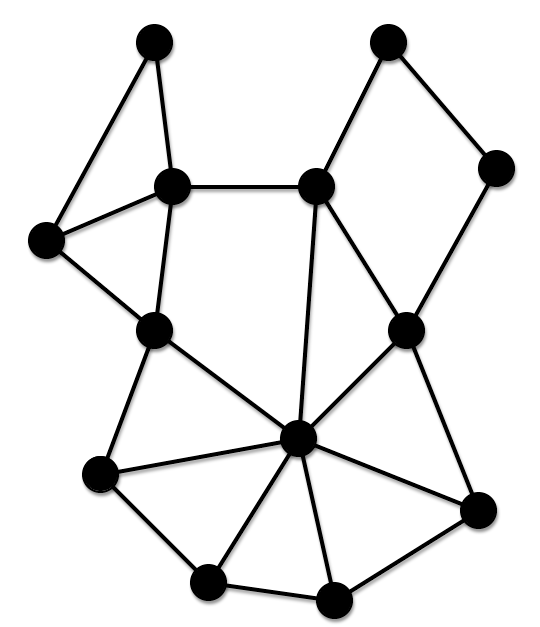
\includegraphics[width=0.5\textwidth]{img/p2p-unstructured}
\caption{Example of unstructured P2P network}
\label{fig:p2p_unstructured}
\end{figure}

%definition
The unstructured systems does not have a strong structure topology. The nodes
establish links in a semi-arbitrary way. Usually, they organize as a hiearchical or a
plain graph.

%advantage
Their main advantage is that they can achieve certain grade of node anonymity.

%disadvantage
The downsize of this type of systems is that searches can end in false
negatives and have a bigger cost in comparizon with structured networks. This
is because the search algorithms do not pass through every nodo inside the
graph.

They are commonly used to share files, using the anonymity of the user to
distribute any tipe of file through the net.

% examples
There are many implementations of unstructured networks:
Gnutella~\cite{oai:CiteSeerXPSU:10.1.1.61.7302}, 
BitTorrent~\cite{bittorrent}, 
%Freenet~\cite{freenet}, 
%Overnet~\cite{overnet}, 
among others. Each one use differents ways to organize the nodes, some using a
node hierarchy to facility the searches in the the network, and others simply
does not count with a search method (BitTorrent).

\paragraph{P2P Unstructured Data Storage}
\label{sec:p2p_unstructured_storage}

This systems storage system does not relate with their network topology, and
does not have a fixed procedure for it. In general, when a node asks for data
and copy it, the network use his copy to distribute it with more nodes in the
system. Each user can decide if he want to share a data or not with the system.
That can make some data of the system go unavailable, and the network by its
own does not have a way to control this.


\paragraph{P2P Unstructured Data Search}
\label{sec:p2p_unstructured_search}

There are many ways to make search inside this type of networks. Some of them
are:

\begin{itemize}
    \item \textbf{Flooding}: 
Each node tries to forward every message to every one of its neighbours except
the source node. To avoid som wasted duplicate deliveries and infinite loops,
each message has a \textit{Time To Live} (TTL) that limits the amount of times
that it can be forwarded. This type of searches has a cuadratic cost of network
messages, of order O($N^2$), were N is the number of nodes that can route data
inside the network.
    \item \textbf{K-Random Walk}: Similar to the \textit{flooding} method, with
the difference that each node chooses a number K or a fixed percentage of his
neighbours and forwards the message to the ones that were chosen. When a node
with the required information is found, it responds with a QUERY\_RESPONSE
message following the same way that the Random Walk used to reach him, back to
the original node that started the search. The message cost of this searches
depends of the value of K, approaching:

\numberwithin{equation}{subsection}
\begin{equation}
\label{eq:krandomwalk}
 C = 2 + TTL +
\sum_{i=0}^{TTL} K^i
\end{equation}

\end{itemize}

A way to reduce the message cost in this type o searches, \textit{caching}
techniques can be used, saving the location of the files shared in the network
as they are distributed in it.

\subsection{P2P Structured Networks}
\label{sec:p2p_estructured}

\begin{figure}
\center
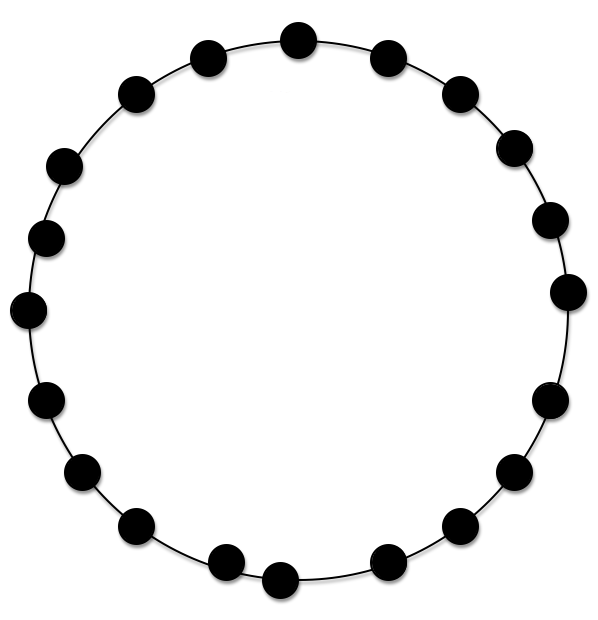
\includegraphics[width=0.5\textwidth]{img/p2p-structured}
\caption{Example of structured network}
\label{fig:p2p_estructured}
\end{figure}


%definition
The structured networks have a strong topology structure. While most of them
use ring structures, other base his topology in binary trees or other
structures to organize.

%advantages
The main advantage of this systems are they searches. The data search does not
suffer of false negatives, and is more efficient in message cost and response
time than the unstrucutred ones. 

%disadvantages
As the nodes can be found and traced easily with a query, user anonymity is harder to
achieve in this type of systems.  The applications that want to maintain user
anonymity from his users, this is one of the main reasons to not use this type
of systems.

% examples
The vast mayority of structured P2P systems use distributed hash tables
(DHT)~\footnote{http://en.wikipedia.org/wiki/Distributed\_hash\_table} as
structural base for the search and storage system~\cite{BalakrishnanEtAl03}.
CHORD~\cite{conf:hotos:DabekBKKMSB01},
PASTRY~\cite{oai:CiteSeerPSU:441779} and 
OpenDHT~\cite{Rhea:2005:OPD:1080091.1080102}
are some of the systems that are DHT based.

\subsubsection{Chord}
\label{sec:chord}

Is a protocol for the implementation of DHT networks that relates a key with
each node. It is design to work in decentralized networks without the use of
special nodes (like super-nodes to help the realization of queries). His
architecture is made to have a basic operational cost proportional to $log(N)$,
with $N$ being the number of nodes in the network.

The protocol takes in consideration that nodes can be inactive or away one
moment or another. Uses the SHA-1 function to asign identifiers to each node
and keys in the system. The Chord protocol dynamically allocates identifiers to nodes that
join or leaves the network. The rest of tasks and services that the system
would need - like user identification, storage, interfaces, etc.- are
responsability of other implementations of a higher abstraction level than the
Chord protocol itself.

\label{sec:chord}
\begin{figure}
\center
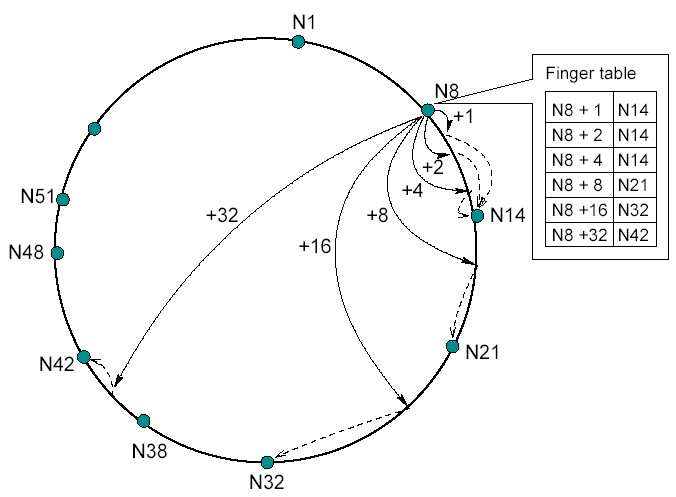
\includegraphics[width=0.5\textwidth]{img/chord-search}
\caption{Chord Routing}
\label{fig:p2p_estructured_chord_search}
\end{figure}

\paragraph{Chord Data Storage}
The network data is stored in the closest node succesor of the hash key of the
data. The network searchs are made querying the closest succesor
nodes that the node has in his \textit{finger table}.
The id key $k$ is assigned to the node id $k$ if this one is active in the
network. If $k$ is not available at that moment, it search for the first node
successor to $k$ that is active and the key id is assigned to him. This
sustitute node is denominated \textit{succesor of $k$}.
The more close a node id is from other, the more far away phisically are the
nodes distributed, giving the network a better resilience to errors.

\paragraph{Chord Information Search}
Key-value pairs are generated using a hash function over each participant of
the network.  Each node register a routing table called \textit{Finger Table}.
In the \textit{Finger Table}, each node register his $i$ successor nodes, each
one being the closest successor to $\theta + 2^{i-1)}$. 
In a search, the number of nodes that a query needs to reach is of order
$O(log(N))$.
The problem that Chord has is that it does not maintain a correlation
between the logical locality of the nodes and their geographical positioning. This
produces that the network communication ocurrs between nodes very close
logically, but very far phisically in the network. While some
optimizations using different heuristics exists to make it better, the locality
problem is not completelly fixed.

\subsubsection{Pastry}
\label{sec:pastry}
Pastry is a protocol for the DHT implementation. It defines how the node keys id
are distributed and how to find the node responsible of the storage of a key.

\paragraph{Pastry Data Storage}

The data storage is made applying the same hash function used to assign node
identifiers (\textit{nodeID}) to the data filename. This results a key, wich is
mapped to a single node. In Pastry, the file is stored in the node that has the closest nodeID to
the to the data's key.

Exists many replication technices that manage and distribute copies of the file
in the network. The distribution of the copies is made using the closest nodes
to the chosen node. Using this, if the node in charge of the storage of thefile
is missing, the file can still be recovered from his replicas. Also, thanks
to the hash algorithm used, the replicas that are nearby inside the network are
in reality distributed far geograficaly, improving the data availability
in the system.

\paragraph{Pastry Data Search}

In Pastry, to have an efficient search, each node maintains three data sets:
a routing table, a leafset and a neighbor set.
The leafset is a the set with the closet nodes to the local node, in both
directions of the circle. It serves to maintain the network consistency and
shorten the searches.

The neighbors set are the $m$ closest nodes by the metrics used in the network.
While they are not used by the search algorithm, they helps to maintain the
routing table.
%La búsqueda de información depende del protocolo de red utilizado.
The routing table has a row for each assigned address block. The blocks are
form dividing the nodeID of the local node in digits of $b$ bits. This
generates a numeric system in base $2^b$. In that way, starting at the client,
the nodes are grouped by their number of digits in common in a prefix of the
local node's nodeId and the other node. The table stores in each row the
address of the closest know node, fulfilling the prefix condition of that row.

The messages can be sent to any address in the key space, regardless of whether
the node exists or not. The content is sent through the network until it reaches the node with the given ID (or the closest one, if the exact one does not exist). When a node recieves or sends a message, it checks the leafset searching for a direct route. If it does not find one, it sends the message to the known node in the routing table that has  more prexifes in common with the objective. This makes sure that the message will shorten the distance at each step in the search, reaching always the node with the closest nodeID to the objective.

In~\ref{fig:p2p_pastry_routing} we can see an example of the routing algorithm used in Pastry when sending a message.

\begin{figure}
\center
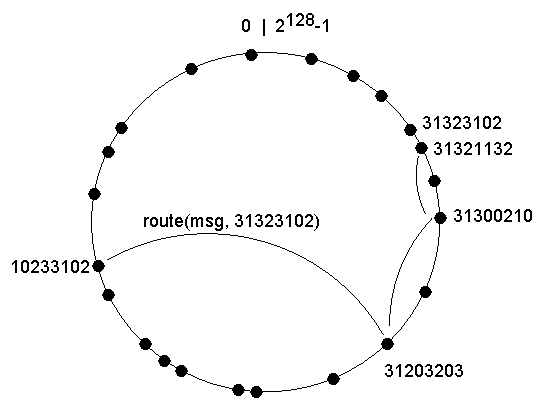
\includegraphics[width=0.6\textwidth]{img/pastryrouting}
\caption{Pastry message routing}
\label{fig:p2p_pastry_routing}
\end{figure}


The search is based in the \textit{lookup(key)}~\cite{BalakrishnanEtAl03} function.
This function takes a \textit{key} and searchs inside of the network a node with
the closest nodeID to the key. If the data exists in the network, the lookup
function returns the node that has it. An important feature of searches in DHT
like Pastry, is that the cost in number of messages is of order $O(log(N))$,
where $N$ is the total number of nodes in the system. Also, it is
\textit{decidable}, meaning that if the data exists in the network, this data
can be found if requested. Other characteristic of the system is his natural
load balancing. The routing algorithm ensures that the request will pass through
a leafset node before reaching the root node, making available for the leafset
node to respond to the request, balancing the load of the request in its
leafset nodes.


%
%
%\subsubsection{CAN}
%\label{sec:can}
%%The “Content Addressable Networks” (CAN) [22] work is being done at AT&T Center for Internet Research
%%at ICSI (ACIRI). In the CAN model, nodes are mapped onto a Æ -dimensional coordinate space on top of
%%TCP/IP in a way analogous to the assignment of IDs in Tapestry. The space is divided up into Æ dimensional
%%blocks based on servers density and load information, where each block keeps information on its immediate
%%neighbors. Because addresses are points inside the coordinate space, each node simply routes to the neighbor
%%which makes the most progress towards the destination coordinate. Object location works by the object
%%server pushing copies of location information back in the direction of the most incoming queries.
%%There are several key differences between CAN and Tapestry. In comparison, Tapestry’s hierarchical overlay
%%structure and high fanout at each node results in paths from different sources to a single destination con-
%%verging quickly. Consequently, compared to CAN, queries for local objects converge much faster to cached
%%location information. Furthermore, Tapestry’s use of inherent locality paired with introspective mechanisms
%%means it allows queries to immediately benefit from query locality, while being adaptive to query patterns
%%and allowing consistency issues to be handled at the application layer. CAN assumes objects are immutable,
%%and must be reinserted once they change their values. Finally, Tapestry node organization uses local net-
%%work latency as a distance metric, and has been shown to be a reasonable approximation of the underlying
%%network. CAN, however, like Chord, does not attempt to approximate real network distances in their topol-
%%ogy construction. As a result, logical distances in CAN routing can be arbitrarily expensive, and a hop
%%between neighbors can involve long trips in the underlying IP network. The main advantage a CAN has is
%%that because of the simplicity of the node addition algorithm, it can better adapt to dynamically changing
%%environments such as sensor networks.
%%In summary, Pastry, Chord and CAN are very similar to Tapestry in their functionality and run-time proper-
%%ties. In particular, Pastry is the closest analogy offering “locating and routing” to an object, where Chord and
%%CAN both focus on providing distributed hashtable functionality. Because Pastry controls replica placement,
%%and Chord and CAN are not optimized for large objects, Tapestry is the only system which allows the user
%%to control the location and consistency of the original data, allowing the system to manipulate and control
%%only references to the object for performance. It is also noteworthy that Tapestry and Pastry have natural
%%correlation between the overlay topology and the underlying network distance, while CAN and Chord may
%%incur high physical hop counts for every logical hop.
%
%\begin{figure}
%\center
%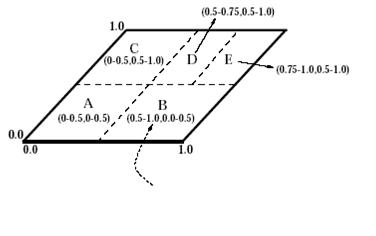
\includegraphics[width=0.6\textwidth]{img/can_structure}
%\caption{Ejemplo de la estructura de CAN}
%\label{fig:can_structure}
%\end{figure}
%
%\paragraph{Almacenamiento de datos}
%En CAN (\textit{Content Addressable Networks}) el espacio de nombres es
%dividido en bloques dimensionales~\ref{fig:can_structure} basándose en la densidad y carga de
%información de los nodos. CAN asume que los objetos son inmutables, y deben ser reinsertados
%una vez que han cambiado sus valores.
%
%\paragraph{Búsqueda de la información}
%Cada bloque mantiene información sobre sus vecinos
%inmediatos. Debido a que las direcciones son puntos dentro del espacio de
%coordenadas, cada nodo simplemente enruta hacia el vecino que realiza el mayor
%progreso frente al del vecino. Una vez que el objeto es encontrado, la
%información es enviada de forma inversa hacia la dirección de más consultas
%realizadas. Al igual que Chord, no mantiene
%correlación entre el espacio de nombres utilizado y la distancia física de los
%nodos, pero su simplicidad le permite adaptarse mejor a ambientes de alto
%dinamismo.
%
%%\subsubsection{Skip Graphs}
%%\paragraph{Almacenamiento de datos}
%%\paragraph{Búsqueda de la información}
%
%\subsubsection{Tapestry}
%\label{sec:tapestry}
%
%%PAST [11] is a recent project begun at Microsoft Research focusing on peer-to-peer anonymous storage.
%%The PAST routing and location layer, called Pastry [10], is a location protocol sharing many similarities
%%with Tapestry. Key similarities include the use of prefix/suffix address routing, and similar insertion/deletion
%%algorithms, and similar storage overhead costs.
%%There are several key differences that distinquish Pastry from Tapestry. First, objects in PAST are replicated
%%without control by the owner. Upon “publication” of the object, it is replicated and replicas are placed on
%%several nodes whose nodeIDs are closest in the namespace to that of the object’s objectID. Second, where
%
%%Tapestry places references to the object location on hops between the server and the root, Pastry assumes
%%that clients use the objectID to attempt to route directly to the vicinity where replicas of the object are kept.
%%While placing actual replicas at different nodes in the network may reduce location latency, it comes at the
%%price of storage overhead at multiple servers, and brings with it a set of questions on security, confiden-
%%tiality, and consistency. Finally, Pastry routing’s analogy of Tapestry’s “surrogate routing” algorithm (see
%%Section 3.3) provides weaker analytic bounds on the number of logical hops taken. In Tapestry, we have
%%analytically proven, well-defined, probabilistic bounds in routing distances, and are guaranteed to find an
%%existing reachable object (see Section 3).
%
%\paragraph{Almacenamiento de datos}
%Comparte muchas similitudes con Pastry, como su ruteo basado en el
%prefijo de las direcciones, algoritmos similares para la  inserción y borrado y
%costos de almacenamiento de la información.
%Tapestry usa claves numéricas de 160 bits, generadas mediante SHA-1, como
%identificadores tanto de nodos como de objetos dentro de la red. Éstos
%identificadores suelen representarse en formato hexadecimal, siendo más
%próximos dentro del espacio de identificadores contra más dígitos tengan en
%común. 
%Los objetos son publicados enviando un mensaje de publicación hacia el nodo
%raíz correspondiente al hash del objeto. Cada nodo del camino guarda un puntero
%hacia el objeto. Los links redundantes son priorizados por latencia y/o
%localidad.
%
%%De ésta forma, objetos son encontrados realizando consultas hacia la
%%raíz del objeto, en donde cada nodo por el camino revisa sus punteros y
%%redirige la petitición apropiadamente.
%
%%Participants in the network can publish objects by periodically routing a
%%publish message toward the root node. Each node along the path stores a pointer
%%mapping the object. Multiple servers can publish pointers to the same object.
%%The redundant links are prioritized by latency and/or locality. Objects are
%%located by routing a message towards the root of the object. Each node along
%%the path checks the mapping and redirects the request appropriately. The effect
%%of routing is convergence of nearby paths heading to the same destination.
%
%
%\paragraph{Búsqueda de la información}
%
%Un mensaje busca primero un nodo cercano que tenga en común con la clave
%del destino el mismo número en el dígito de menos peso, incrementando
%paulatinamente la parte común hasta encontrar el nodo existente más cercano,
%como se puede visualizar en la figura~\ref{fig:bayeux_routing}.
%
%Para dirigir los mensajes a su destino, Tapestry usa tablas de enrutamiento
%locales en cada nodo, conocidas como \textit{neighbor maps}. La tabla contiene
%múltiples niveles, en donde cada nivel representa un sufijo coincidente hasta
%un dígito. Un nivel dado contiene varias claves, las cuales varían solo en el
%número en la posición indicada por la tabla, similar a la tabla de ruteo
%utilizada por Pastry.
%
%Una búsqueda realiza $O(log_B N)$ saltos en una red de tamaño $N$ y espacio de
%nombres de base $B$. Para un mejor nivel de tolerancia de fallos, se mantiene
%una lista de $c$ links secundarios, de tal forma que la tabla de ruteo posee
%un tamaño de $c B log_B( N)$.

%\red{OTRAS REDES}


\subsection{P2P Networks and User Identification systems}

The work will be based in structured P2P networks, because unstructured
systems does not have the desired properties for the implementation of a
identification system. 

Debido a las propiedades poco favorables de las redes P2P no-estructurados para la implementación de una red
social, una red P2P estructurada como base sería lo más adecuado para su
implementación, por lo que el estudio a continuación se centrará  principalmente
en los sistemas Peer-to-Peer estructurados.

\subsubsection{Implementaciones de redes sociales P2P}
No existen actualmente implementaciones de redes sociales P2P,
existiendo sólo propuestas teóricas para una implementación futura. Un proyecto
que actualmente se encuentra trabajando para lograr esto es
PeerSoN~\footnote{http://www.peerson.net}~\cite{buchegger:peerson, buchegger:2009:pps:1578002.1578010}.

\paragraph{PeerSoN}
PeerSoN presenta un prototipo de estructura para redes sociales
Peer-to-Peer, buscando asegurar la privacidad de los usuarios y potenciar la
comunicación directa entre cada usuario.
Su arquitectura está basada en 2 capas, una para la búsqueda y otra para el almacenamiento de la
información. Considera la asignación de identificadores únicos para cada
usuario, procedimientos de entrada, envío y obtención de archivos y el manejo
de mensajes asincrónicos.

La capa de almacenamiento consiste en los peers en sí, los cuales, una vez
encontrados por la capa de búsqueda, pasan a juntar y enviar la información
directamente entre sí, distribuyendo réplicas de éstos
en la red para aumentar la disponibilidad de los datos. 
PeerSoN~\cite{buchegger:peerson} basa su seguridad en cifrado simétrico y asimétrico. La
información primero es cifrada usando una llave simétrica, y luego esta
llave es cifrada con las llaves públicas de los recipientes. Los
identificadores de los usuarios son cifrados junto con las llaves
simétricas, siendo todo enviado con la información cifrada.

 Por último, para la capa de búsqueda usan las capacidades de almacenamiento,
ruteo y recuperación de información de
OpenDHT~\cite{Rhea:2005:OPD:1080091.1080102}.

%#peerson
Dentro de sus debilidades se encuentran un sistema de seguridad y de búsquedas
muy básicos, sin abordar las problemáticas que pueda tener en una
implementación real del sistema. Su sistema de cifrado requiriere para poder compartir
un dato a grupo una cantidad de procesamiento proporcional a la
cantidad de usuarios. Además, en caso de modificación del grupo, se requeriría
el recifrado de todos los archivos compartidos entre sí, con todos los
costos que esto significaría. En el caso del sistema de búsqueda, al basarse en
un DHT sin mecanismos adicionales, no permitiría búsquedas complejas o de más
de una dimensión, dificultando el proceso de establecimiento conexiones entre
la red.

\paragraph{Safebook}
Safebook~\cite{conf_wowmom_CutilloMO11} es un propuesta la formación para una
red social que utiliza dos principios de diseño: descentralización y uso de la
confianza con los usuarios de la vida real. Su arquitectura la organiza
separándola  en 3 niveles: red social (\textit{social network}, SN), aplicación
(\textit{application services}, AS) y transporte y comunicación
(\textit{communication and transport}, CT). El primer nivel es provisto por la
representación digital de los miembros y sus relaciones, la capa da aplicación
corresponde a la infraestructura de la red social y por último la capa de
comunicación que corresponde al Internet. 
De ésta forma, un usuario es representado como un \textit{host node} en la
Internet, un \textit{peer node} en la capa P2P, y un miembro o usuario en la
red social.
Uno de sus objetivos es ser resistente a gran parte de los posibles ataques a
redes sociales~\ref{sec:ataques}.

 Confía en matryoshkas que proveen el almacenamiento de la información, perfiles de la obtención de la información
y ofuscación de la comunicación. Una matryoshka consiste en un set de nodos
agrupados en varios anillos concéntricos, los cuales se organizan acorde al nivel de confianza que el
nodo, asociado con la matryoshka, tiene hacia los nodos de cada anillo. El
anillo más interior es el más confiado y estaría formado por los ``amigos'' del
nodo. Este sería el responsable  de almacenar la información replicada del nodo
asociado con la matryoshka. Las capas más cercanas almacenan la información
publicada de forma encriptada y no-encriptada, pero la información privada es
almacenada por el mismo dueño y no es replicada hacia los anillos. 

Para la autenticación del usuario, utiliza un servicio de identificación
confiable para proveer a cada nodo identificadores únicos: un \textit{identificador del
nodo} y un \textit{seudónimo}.
Acuerdo a~\cite{springerlink_10.1007_978-3-642-14282-6_7}, un esquema simple de encriptación grupal es usada para la
encriptación, y usuarios obtienen llaves oportunamente para desencriptar la
información publicada. El dueño debe explícitamente autorizar y volver a publicar al
anillo interior cada mensaje escrito por otros usuarios.
La anonimidad en Safebook es obtenida usando un ruteo de múltiples saltos. Una
tabla de hash distribuida mantiene punteros a los nodos pertenecientes al
anillo más lejano de la matryoshka. Las peticiones entrantes son ruteadas desde
el anillo más lejano hacia el centro de la matryoshka. Los mensajes son
encriptados en cada salto usando criptografía asimétrica.

La búsqueda de información se realiza a través de consultas recursivas en el
sistema P2P a través del DHT. Para ello, el nodo realiza una consulta
por la información del usuario objetivo, requiriendo el conocimiento previo de
los identificadores de éste. De ésta forma, consulta al nodo responsable del
identificador de ese usuario por la lista de nodos de entrada de la
capa más lejana de la matryoshka del usuario objetivo. Por último, la consulta
prosigue reenviandose a través de los nodos de cada capa de la matryoshka, hasta
llegar al centro de la misma. La información requerida llega de vuelta a través
invirtiendo el camino de llegada de la consulta.
No contempla un sistema de búsqueda adicional al provisto por el DHT.

Los problemas principales detectados de este sistema se encuentran en la
disponibilidad de la información, problemas de escalabilidad al depender de
sistemas externos para el ingreso de nuevos usuarios a la red y carencias en
los métodos de búsqueda y recuperación de la información.
Esto es debido a que el almacenar réplicas de los datos personales entre los amigos más cercanos
puede generar problemas de disponibilidad de los datos en los momentos en que
éstos no se encuentren en linea. Para la identificación requiere de un servicio
externo centralizado  que pueda ser confiado para la asignación de ID únicas.
Por último, la transmisión de mensajes a través de la red se realiza
anonimizando al que envía y recibe el mensaje, aumentando el costo y tiempo de
envío de cada dato por cada salto que de entre nodo y nodo.


\label{sec:soa_p2p_user_identification}
\section{P2P identification schemes}

%% INTRO
 As P2P systems grow in complexity, a way to identify individual users among the
network nodes is needed. To attain this, additional protocols are needed to
ensure that the identity of a node corresponds truthfully to the user it
proclaims to be. A basic way to identify a registered user is by the use of
a private/public encryption scheme. While this can work in simple environments
with a few known users, to allow registration over the network a way to store
the user keys and verify their authenticity is needed.
Next we are going to detail an identification scheme that allows user
registration and identification using the user's username and password.

%% END INTRO

% TODO for revision
The subject of securely establishing stable identities in P2P
systems has been previously studied, for instance, by Aberer,
Datta and Hauswirth~\cite{1318567}. The need for identities mainly arose
from technical concerns, such as handling dynamic IP address
assignment, or avoiding Sybil attacks~\cite{the_sybil_attack}. Authentication of a
node is done via a signature key, automatically generated and
stored on the node.

Traditionally, P2P networks identified the different nodes that compose the
system, but not the user behind each one of them as a different being.
As P2P systems grew in complexity, the need to identify users inside the
network arose.

% TODO for revision
Some P2P storage systems also use techniques which are
related to ours. For example, the DHT-based systems GNUnet
and Freenet use keyword strings to derive a public-private key
pair. The private key is used to sign data and the hash of
the public key to identify the data in storage. Both of
these systems use a keyword string as a seed to a pseudo-random number
generator that produces the key pair~\cite{clarke2010private},~\cite{Bennett03anencoding}.
Knowing only the memorable keyword string the user can
store and retrieve information.

% TODO for revision
Related to forgotten passwords, recovery of information in a
P2P scenario has been studied by Vu et al.~\cite{5380695} who proposed
a combination of threshold-based secret sharing with delegate
selection, and encrypting shares with passwords.
Frykholm and Juels~\cite{Frykholm:2001:EPR:501983.501985} proposed a password-recovery
mechanism based on security questions very similar to our
protocol for the same task. They offer better information-theoretic security properties, something not applicable to our
scenario. We address the subject of password change, which is not applicable to
their scenario, although their proposal could be extended to support password
change using our techniques.


%\subsection{Plain PKI scheme}
\subsection{Peerson username/password scheme}

Kreitz et al.~\cite{kreitz2012passwords} present a suite of protocols for password
authentication in P2P networks: account registration, login, password change,
remembered logins, logout from a remote device, and password recovery.
Password authentication is based on standard cryptographic techniques and can
be used with standard P2P components. 

It relies on the safe storage, distribution and retrieval of a a)~\textit{login information
file}, a b)~\textit{device login info file} and a c)~\textit{key store
file}~\ref{fig:p2p_peerson}.

\begin{enumerate}[a)]

  \item The login information file stores encrypted files and a
plain text. The encrypted files are: the user session information (\textit{devmap}), a
cryptographic key for write authentication ($K_W$), and the \textit{filename of the
key store file} ($f_{KS}$) along with the \texit{symmetric key} used to encrypt and
decrypt the \textit{key store file} ($K_{KS}$). The plain text is a random byte string used as a \textit{salt} to generate the user private key to
decrypt the first bundle of files. 

  \item The \textit{key store file} ($F_{KS}$) stores all the private keys used to identify the
    user in the system services. This file is encrypted by the $K_{KS}$ key.

  \item The device login information file only stores the filename of the key
    store file and the $K_{KS}$ key, both of which are encrypted by a $K_{DL}$ key
    stored in the \textit{devmap}.
\end{enumerate}

\begin{figure}
\center
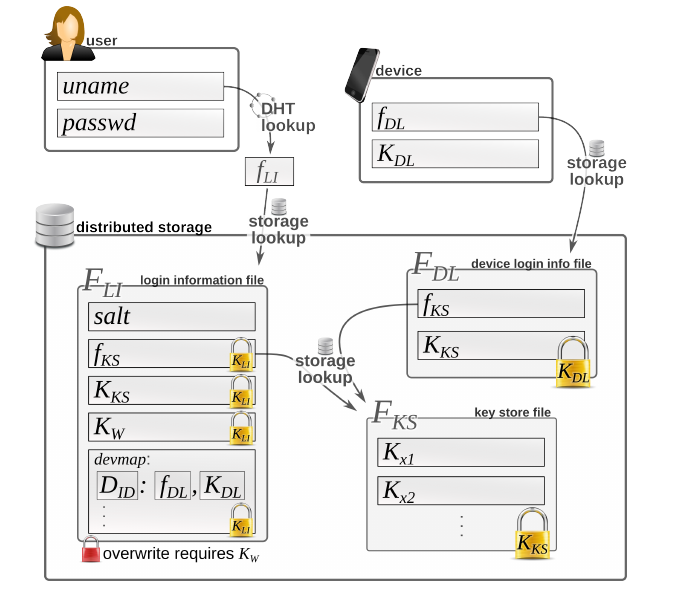
\includegraphics[width=12cm]{../img/password_peerson}\\
\caption{Peerson scheme storage locations (boxes) and login procedure (arrows) }
\label{fig:p2p_peerson}
\end{figure}

Their protocols are as follows:
%
%% introduction of identification schemes. Par 2: proposed username/password identification schemes. Part 3: securing the network protocols. Part 4: Pending issues.
\subsubsection{Account registration}
%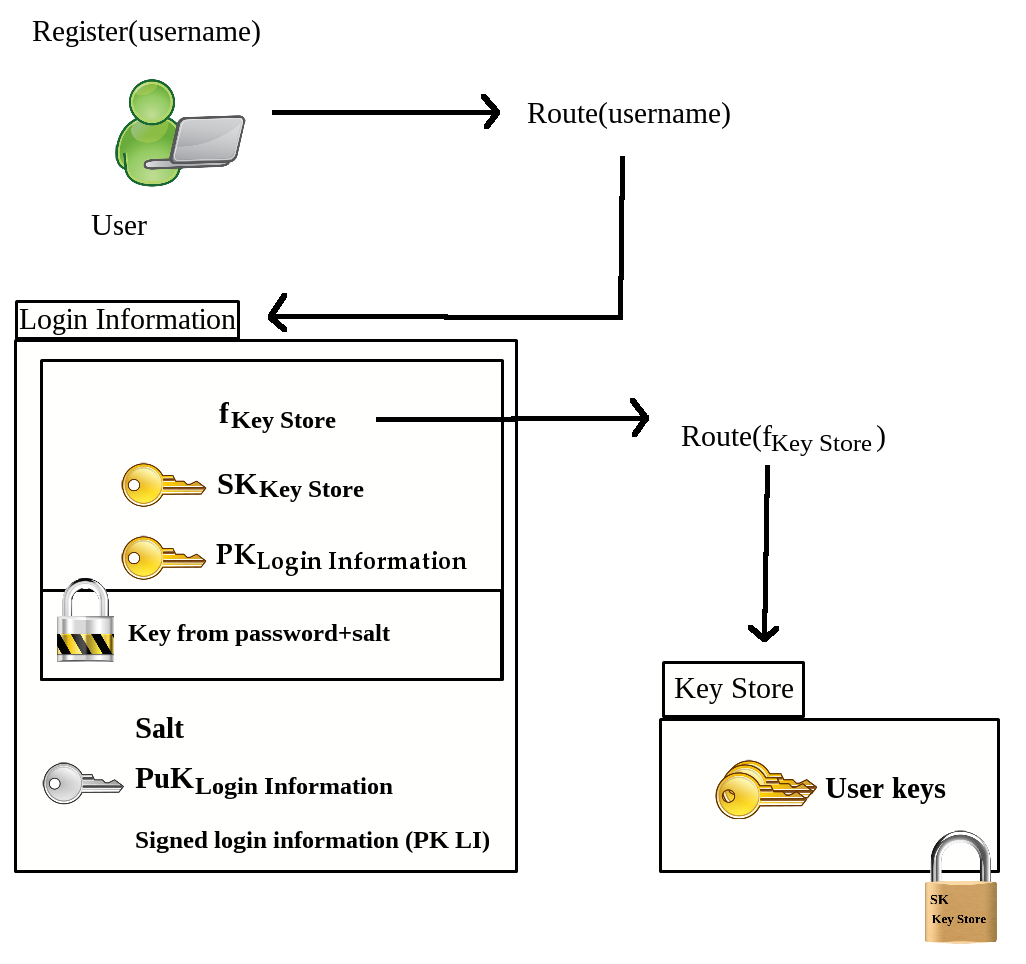
\includegraphics[width=14cm]{../img/user_registration}\\

To register a new user account, the user first
has to choose a \textit{username} and a \textit{password}.
In the key-based authentication, the user creates a \textit{key store
file} $F_{KS}$, containing all the
keys used by the P2P application the user wants to login to.
The user generates a cryptographic key to authenticate the write operations
that will be made in the file. The cryptographic key is then stored with the
other keys in the \textit{key store file} $F_{KS}$.

% encryption and store of the key store file
The user then creates a \textit{symmetric key} $K_{KS}$, which is used to
encrypt the file content. Then the ciphertext
is put into storage, obtaining a \textit{filename} $f_{KS}$ for it. Now, the user
creates a \textit{login information file} $F_{LI}$ by creating a random
byte string, or \textit{salt}, and deriving a \textit{symmetric key} $K_{LI}$ from the user
\textit{password} and the \textit{salt}.
Using the new \textit{ symmetric key} $K_{LI}$, the user encrypts the
filename $f_{KS}$,
the \textit{symmetric key} $K_{KS}$ and the cryptographic key to
authenticate the write operations $K_W$.
 The \textit{salt} and the three encrypted values are put
into storage, obtaining a filename $f_{LI}$ . The \textit{salt} is stored
in plaintext, so that the user can later derive the decryption
key $K_{LI}$ by only providing the password. Finally, the user
performs the write-once operation \textit{put} on the DHT, with
username as key and $f_{LI}$ as value.

%unique username
If the username was taken,
the user is prompted for a new username.

%finish
Once all operations
have succeeded, the user is registered in the system.


\subsubsection{login}


The user uses his username to find and retrieve his \textit{login information
file} $F_{LI}$. Then, using his \textit{password} and the \textit{salt} included in the
\textit{login information file} $F_{LI}$, obtains the filename
$f_{KS}$ used to
route back to where the \textit{key store file} $F_{KS}$ is stored.  Lastly, he uses the
\textit{symmetric key} $K_{KS}$ to decrypt the \textit{key store file}
$F_{KS}$ and recover his user keys.

\subsubsection{Password change}
%To change the password, the user has to rewrite his \textit{login information
%file}.


Before the user can change his password, he must login using his password to
obtain the $K_{LI}$ . With this information, the password change can be
completed. The user is asked for a new password and a new \textit{salt} is
generated. The key-derivation function is used to generate a new key
$K_{LI}^{new}$
for the login information file. Then, the content of the \textit{key-store
file} is
retrieved and decrypted (with the old key). A new key $K_{KS}^{new}$ is generated and
used for encrypting the key-store content again before it is saved in the
storage system. The storage of the key-store content returns a new filename $f_{KS}^{new}$.
Finally, the \textit{login information file}
is updated: $f_{KS}^{new}$, $K_{KS}^{new}$, the write credential $K_{W}$ as well as a new empty
device mapping file \textit{devmapnew} are encrypted with the new key $K_{LI}^{new}$.
  Together with the new \textit{salt}, this ciphertext is written to the distributed
storage, using the reference $f_{LI}$ and the credential $K_W$, to authenticate the
write operation. Lastly, the keys stored in the key-store should be updated by
the application using the P2P protocol.  At this point, old device login
information files can also be deleted from the
storage to reclaim space.

\subsubsection{Logout}
%The system does not have something like a "session" to maintain; the only way
%to identify an user is by his keys that are obtained by the identification
%process.

To logout from the system, the user does not have to interact
with the DHT or the storage system. Simply wiping the local
cache from application data and all key material restores the
pre-login state. If the user chose to remember the login on a
device, the corresponding \textit{device login information file} $F_{DL}$
can also be deleted from storage.
 A problem related to logging out is revoking remembered
credentials on another device, e. g., a user’s stolen phone. To
accomplish this, they first run the password change operation,
which locks out all devices with remembered logins, because
the key store key $K_{KS}$ changed (as well as the filename $f_{KS}$).
Next, we use the device mapping file \textit{devmap} to inform all devices
about the new key (and filename), except the device that is to
be revoked. To inform a device about the change, we update
the corresponding values in the device’s \textit{login information file}
 $F_{DL}$ which can be accessed from the device by using the
locally stored credentials.

 After running the password change
operation, all devices that should not be revoked and that have remembered
logins (and therefore are referenced in the \textit{devmap}) are
processed. The \textit{device login information filename} $f_{DL}$ and its key $K_{DL}$ are read,
and the new key store key $K_{KS}^{new}$ and filename $f_{KS}^{new}$ are written to the
\textit{device login information file} $F_{DL}$, encrypted under the device key $K_{DL}$.
Finally, the modified \textit{devmap} is saved back to the \textit{login
information file} $F_{LI}$.


\subsubsection{Forgotten passwords and password-recovery mechanisms}
  %- HUGE danger
  %- Security questions
  %- threshold-based secret sharing with delegate selection and encrypting
  %shares with passwords

%%%%%%%%%%%%%   Peerson Passwords in P2P networks %%%%%%%%%%%%%
%An important part of password-based logins is the possi-
% bility for users to recover their accounts if they forget their
% passwords. We refer to this as a password recovery mechanism.
% The goal of a password recovery mechanism is to provide a
% secondary way of authenticating the user. There are a number
% of password recovery mechanisms used in practice. In our
% experience, three of the most common ones are password
% hints, security questions, and e-mail based recovery. Other
%
%approaches (beyond the scope of this paper) include vouching
%for identity by social contacts [21], or using trusted devices.
% Password hints means that the user may enter a hint at
%the same time as she sets this password. The hint will be
%displayed to her if she forgets her password, and should be
%selected such that it helps her recall her password, but does
%not make it significantly easier for someone else to guess it.
%The hint is not truly a secondary authentication mechanism,
%but rather a means to recovering the original password-based
%authentication mechanism. A basic version of password hints
%would be straightforward to implement in our system: the
%hint can be stored in plaintext in the login information file.
%Security questions and e-mail based password recovery are
%more complex to adapt. We described their implementation in
%detail after listing requirements.
%
% As in Section IV for the login procedure, we define a set of
%functional requirements for password recovery, based on the
%ISO 27002 standard [19] as follows. We also augment the list
%with requirements of our own (preceded by a star).
%establish methods to verify the identity of a user prior to
%•allowing the user to choose a new password
%communicate with those affected by or involved with
% - recovery security incidents
% - have procedures to allow recovery and restoration of
%business operations and availability of information in a
% time-scaled manner
%a legitimate user should be able to recover lost (forgotten)
% - or broken (device’s) keys
% - the recovery procedure should allow a user to set a new
% password, not reveal the old password
% - the process of recovery should be easy to use
% - sensitive information for recovery should be kept secret
%
%Our protocols support these requirements.

%% The sole exception
%% is that if a password is reset via security questions alone, the
%% system would not “communicate with those affected” (e.g.,
%% send an e-mail notification that the password had been reset,
%% as is common in centralized services). We remark that the
%% last item is a property many centralizedstronger than systems
%% provide. In our system, no one learns the answers to a user’s
%% security questions. We consider this to be important, since
%% many systems use similar security questions.
%% 
%%  The operations described in this section imply minor addi-
%% tions to the protocols of Section IV, i. e., invoking the update
%% procedures after each password change (to sustain transaction
%% safety, the updates have to be included in the final write
%% operation of the password change operation).
%% A. Security Questions
%%  Security questions is a password recovery technique that
%% relies on answers to questions the user is asked during regis-
%% tration. The answers should be such that they cannot be easily
%% guessed or researched by an attacker, but still stable over
%% time, memorable, and definite [22]. Rabkin [23] underlines
%% the importance to choose good questions especially in the era
%% of social networks. Frykholm and Juels [12] discuss a related
%% technique that is similar to our adaption of this scheme.
%% %%%%%%%%%%%%%   Peerson Passwords in P2P networks %%%%%%%%%%%%%

Depending on the desired functionality of the network, they propose two
mechanisms to provide user password recovery. The actual implementation
requires small modifications in the protocols seen above.

\paragraph{Using security questions.}

 The protocol assume that the user provides $n$ answers $A_i$ to suitable
 security questions $Q_i$ . In order to recover the password, it is
 required for the user to answer any $k$ out of these $n$ questions
 correctly. The choice of $k$ constitutes an obvious trade-off
 between security and usability. A successful recovery yields
 the key $K_{LI}$ to the login information file, allowing the user to
change the password. The implementation
does not require the user to provide new answers after a regular
 password change. Additionally, the protocol avoids storing the plaintext
 answers to the security questions.
 For the setup of the question based recovery mechanism, the protocol first
create $n$ shares $qS_1, \cdots, qS_n$ of the
 key $K_{LI}$ under an $(n, k)$-secret sharing scheme. For each of
 these shares, it is created a salt $qsalt_i$ , derived a key $qK_i$ from
 this salt and the answer $A_i$, and used it to encrypt the share,
 yielding $qS^{enc}_i$. Furthermore, it is encrypted the key $qK_i$ with
 the login information file key $K_{LI}$, for the update procedure
 described later. Finally, the login information file is extended
 with all questions $Q_i$, the salts $qsalt_i$, the encrypted shares
 $qS_i^{enc}$ and the encrypted keys $qK_i^{enc}$. When recovering, the
 user has to reproduce at least $k$ answers, which together with
 the stored salts can be used to derive $k$ keys $qK_i$, which in
 turn can decrypt $k$ shares $qS_i$.
 When $K_{LI}$ changes (e. g., due to a regular password
 change), we update the recovery information %as in~\ref{sec:}
 for the new key $K_{LI}^{new}$, a new set of shares is created.
 Next, the keys $qK_i$ are decrypted and used to encrypt the new
 shares. Neither the keys $qK_i$ nor the salts $salt_i$ change, so
 the user can still use the same answers for recovery. Finally,
 the updated shares (and re-encrypted keys, to allow further
 updates) are saved back to the login information file.

\paragraph{Email based.}

  In e-mail based password recovery, the user is sent an e-mail
 containing some information, typically a link with a token, by
 which she can reset her password. This link is sent to an e-mail
 address she has registered with her account.
 We adapt this scheme by randomly choosing a number of
 peers, that collaboratively provide this functionality to the user.
 

 It use $(n, k)$-secret sharing to enable password recovery even
 if not all of the involved peers are online when the user wants
 to recover the password.
 To provide persistence of the recovery mechanism independent of a changing key $K_{LI}$ (e. g., due to a password change),
 the result of the recovery process is a recovery key $K_R$ ,
 that always encrypts the current version of $K_{LI}$.
  From the recovery key $K_R$, $n$
 shares $eS_1, \cdots, eS_n$ are generated using $(n, k)$-secret sharing.
 For each share, a random peer $peer_i$ is picked, two salts $esalt_i$
 and $ksalt_i$ are created and a cryptographic commitment $C_i$ is
 derived from the salt $esalt_i$ together with the email. This
 commitment will be used to authorize the user to the peer,
 and bind it to this specific e-mail address. Next, a key $eK_i$,
 to encrypt the share $eS_i$ , is derived in the same way as the
 commitment, but with salt $ksalt_i$. A different salt is needed
 so that the peer cannot decrypt the share (before learning the
 address). The commitment and the encrypted share are stored
 at the peer. The login information $F_{LI}$ file is extended with a
 list of the chosen peers $peer_i$ and the according salts $esalt_i$ ,
 $ksalt_i$, as well as $K_{LI}^{enc}$, encrypted with the recovery key, and
 the recovery key, encrypted with $K_{LI}$ (to allow for password
 changes).

 To recover the password, the user looks up the
 available information in the login information file, including
 the list of peers to be requested for assistance. Each request is
 authorized by the commitment $C_i$, that the peer can derive
 from the salt $esalt_i$ and the e-mail address that the user
 provided. If the request was legitimate, the peer
 sends the encrypted share to the e-mail address. As soon as
 the user collected $k$ answers, he can recover $K_{LI}$ .

 To provide long-term persistence of this recovery mechanism, $K_{LI}^{enc}$
 has to be updated whenever $K_{LI}$ changes.
 
 \paragraph{Combining Approaches}
 Also mentions a combining approach using questions and email recovery, either
sequentially or in parallel.
  By sequential composition, they mean
 that the user must both correctly answer security questions and
 receive e-mail. In parallel composition, either
 mechanism can be used alone to recover the password. The
 latter is achieved by using both systems in parallel.
 For sequential composition, the user picks a uniformly
 random string $r$ of the same length as $K_{LI}$. The user stores $r$ in
one of the mechanisms, and $K_{LI} \bigoplus r$ in the second mechanism, where
$\bigoplus $ denotes the exclusive-OR operation.

  If one recovers both of these, $K_{LI}$ can be computed. If one learns only one
 of the pieces, nothing is gained, as both $r$ and $K_{LI} \bigoplus r$ are
 uniformly random. More generally, to combine $n$ mechanisms
  in arbitrary ways, $(n, k)$-secret sharing can be used. What they
 describe there are two trivial such schemes for $n = 2$.\\



%\section{Keys generation}
%\subsection{Randomly derived}
%  manual backup of the keys
%\subsection{Keys derived from a password}


\subsubsection{Conclusions}

Their proposal describes what is needed to obtain a P2P username/password based
identification system, but they do not go deeper beyond that. They are problems
that are not 

% TODO: IDEAS SPANISH
====== IDEAS IN PROGRESS ======

Un problema importante es que su systema de identificacion falla en la
precencia de nodos maliciosos. Esto es debido a que carece de un sistema que
discrimine a los nodos segun su comportamiento, haciendo que bajo una cantidad
baja de nodos maliciosos el sistema tenga altas probabilidades de falla. A
pesar de que nombran el problema, no proponen soluciones que realmente
solucionen el problema.
 %Por ejemplo, si consideramos el registro de usuarios  

Ademas, considerando que ellos asumen que los tiempos de lectura y de escritura
de la red de almacenamiento distribuida son iguales a los de la consulta por
una llave específica en un DHT.

====== IDEAS IN PROGRESS ======

The problem with the existing protocols is that they do not implement in their
protocols measures against the presence of malicious nodes.
A malicious or byzantine node is any node that does
not behave as expected by the protocol of the system. The presence of this type
of nodes can easily break the security and degenerate the quality of the
service in the whole system.


\label{sec:soa_p2p_trust}
\section{Trust in P2P networks}

At the absence of trusted nodes in a P2P network, additional mechanisms to
attain certain grade of trust between the participants of a transaction are
needed. There are reputation systems that grade each node with a reputation
that can be used to decide if a operation will or not will be made with them,
and accountability systems that detects malicious behavior analizing the
behavior of the nodes in the network. While  detecting malicious behavior with
accountability systems can ward off a variety of attacks, they need to follow
each transaction done in the system, with a high cost associated to them.
 In the following section we are going to
detail a reputation system and a trust model to be of used by the proposed
solution.

%Debido a la ausencia de un control central, las redes P2P est ́
% an expuestas a nodos
%maliciosos, especialmente nodos Bizantinos [13]. Se demuestra en [6] que es
%imposible
%dise ̃
% nar e implementar una autoridad de certificaci ́
% on completamente P2P necesaria para
%realizar certificaci ́
% on basada en un sistema seguro. Adem ́
% as, utilizar un conjunto de
%servidores para este fin, no es una soluci ́
% on escalable. Un 30 % de nodos maliciosos, es
%un valor com ́
% unmente aceptado como l ́ımite m ́
% aximo por la comunidad en investigaci ́
% on
%en sistemas P2P. Por lo tanto, construir confiabilidad en este tipo de redes ha
%llegado a ser
%uno de los problemas de mayor inter ́es en la comunidad P2P.
%Los Sistemas de Gesti ́
% on de Confianza permiten clasificar el comportamiento de un nodo
%de acuerdo a las transacciones que ha realizado con otros nodos en el sistema,
%para poder
%decidir si un nodo es confiable. Las soluciones propuestas se dividen en dos
%grandes
%grupos: Sistemas de reputaci ́on [15] y sistemas de tipo accountability [8]. Los
%sistemas de
%reputaci ́
% on permiten obtener un valor R(X) que indica la probabilidad que el nodo X sea
%honesto. Mientras que los sistemas de tipo accountability permiten detectar y
%exponer el
%comportamiento del nodo en base a registros seguros que almacenan las
%transacciones
%realizadas con otros nodos, los cuales son comprobados peri ́
% odicamente.



\subsection{Reputation systems}
Reputation systems mitigate the problem of malicious nodes in
P2P networks, trying to build trust among the nodes. The key
idea of a reputation system is to predict the future behaviour
of nodes based on feedback about their past transactions [1]. A
transaction is application dependent, for example forwarding a
message in the network, buying an item in e-commerce services,
share or store files, etc. After a transaction, the client node emits
a recommendation that evaluates the behaviour of the other peer.
The aggregation of these recommendations leads to a reputation
value.
A reputation system built on top of a DHT has the ability
to compute a global reputation value for every node. Indeed
all the recommendations about a single node can be handled
consistently at a common location: either by a specific node
or by a set of nodes. Among existing reputation systems for
DHTs, we can cite: PeerTrust~\cite{peertrust}, WTR~\cite{wtr},
Eigentrust~\cite{eigentrust},
PowerTrust~\cite{powertrust} and CORPS~\cite{corps}

Reputation systems have to deal with malicious nodes that:
do not participate, collude with other malicious nodes and
emit false recommendations. There are techniques to mitigate
the impact of these attacks, such as the ones presented in
TrustGuard~\cite{trustguard} and WTR~\cite{wtr}. Nevertheless, to our knowledge,
none of the existing solutions to promote trust in P2P can be
$100\%$ effective in detecting and blocking these attacks.

It's assumed an $5\%$ error in the clasification of trusted nodes.

\subsubsection{WTR}
\label{sec:wrt}
WTR~\cite{bonnaire2009wtr} is a reputation system over a DHT like Pastry~\cite{pastry} and
Chord~\cite{chord}. The probability that a node $X$ is honest is determined by
$R(X)$, with $0 \leq R(X) \leq 1$. WTR calculates the node reputation $R(X)$
using the \textit{recomendations} of the node $X$. When a node $Y$ makes a transaction with
node $X$, the node $Y$ issues a recomendation about the behavior of the node
$X$. The recomendations table~\ref{table:wtr_recomendations} shows how each
transaction is evaluated.
 
  \begin{table}
    \centering
    \footnotesize
    \begin{tabular}{|l|l|l|}
      \hline
      \textbf{Status} & \textbf{Recomendation} & \textbf{Description}\\
      \hline
      Excelent  & $1.00$    & Very good transaction\\
                &           & Service fully completed\\
      Good      & $0.75$    & Good transaction\\
                &           & Some degradations\\
      Neutral   & $0.50$     & Not completed correctly\\
                &           & Could be independent of the node\\
      Bad       & $0.25$    & Transaction not completed.\\
                &           & Maybe a malicious node\\
      Malicious & $0.00$    & Transaction not completed\\
                &           & Fully malicious node\\
      \hline
    \end{tabular}
    \caption{Recomendations in WTR}
    \label{table:wtr_recomendations}
  \end{table}

A set of $M$ nodes manage the reputation and the risk associated to node $X$.
The node ID of the manager $i$ of the node $X$ is
obtained by the function $m_i = SHA^{i}(X)$. Each manager of the node $X$
stores the lists of recomendations emitted about $X$. When a manager recieves a
new request for node $X$, it computes the new reputation value and the risk
value for $X$.
Each manager $m_i$ administers a number of $L$ replicas of the reputation information. In Pastry,
the replicas are stored in the leafset of each node, while in Chord the $r$
successors of each node are used.
The reputation and the risk associated to node $X$ are probabilities. The
reputation of $X$ is the probability for $X$ to be trusted. The risk of node
$X$ represents the risk to make a transaction with node $X$. A risk of $1$
means that doing a transaction with $X$ is really risky, even if $X$ has a very
good reputation.

The reputation of a node in WTR is influenced by the credibility of the nodes
that emitted the recomendations about $X$. The credibility of a node $K$ at a
moment $t$ is denoted by $C_t (K)$:%~\ref{eq:credibility_of_a_node}.

\begin{equation}
  C_t (K) = \left\{
  \begin{array}{l l}
    1, & if R_t(K) \in [0.75 \cdots 1]\\
    0.75, & if R_t(K) \in [0.5 \cdots 0.75]\\
    0.2,  & if R_t(K) \in [0.25 \cdots 0.5]\\
    0.1, & if R_t(K) \in [0.0 \cdots 0.25]\\
  \end{array}\right.
%\label{eq:credibility_of_a_node}
\end{equation}

To calculate the reputation of a node, the system only takes in consideration
the last $m$ recomendations in its recomendations list. This window size $m$ is
a fixed parameter of the reputation system. Also, more weight is given to the
more recent recomendations. 
Being $F_i^k (X)$ the recomendation $i$, emitted by the node $K$ to the node
$X$. Then, the reputation of the node $X$ at the time $t$ is defined by:

\begin{equation}
  R_t(X) = \frac{\sum_{i=0}^{m-1}  log(m-i+1) \cdot F_i^k(X) \cdot C_t(K)}{
\sum_{i=0}^{m-1} log(m-i+1) \cdot C_t(K)}
\end{equation}


The problem with only considering the reputation of a node when doing a
transaction is that:
\begin{enumerate}
  \item A node with a number $n$ of good recomendations, with $n \ll m$ (very
few recomendations), can have a very similar reputation than a node with at
least $m$ recomendations. However, an application could really prefer a node
with a larger history as its reputation is computed with more information, and
is therefore more reliable.
  \item A node that makes good and bad transactions in turns can have a very
similar reputation compared to a node with a more regular behavior. It then can
more interesting for an application to choose a node with a more regular
behavior than a very irregular one.

\end{enumerate}

For these reason is that the \textit{risk} of a node is considered. $J_t(X)$ is
the risk to make a transaction with a node $X$ at time $t$. A risk of 0
means that the reputation for node $X$ is fully reliable.

\begin{equation}
  J_t(X) =  T_1 + T_2
\end{equation}

where

\begin{equation}
  \left\{
  \begin{array}{l}
    T_1 = \alpha \cdot (1-\frac{r}{m}\\
    T_2 = 4 * (1- \alpha) \cdot (1-\frac{\sum_{i=0}^{k} (F_i(X)-\bar{F_i(X))^2})}{r}
  \end{array}\right.
\end{equation}

Where $r$ is the number of available recommendations in the siliding window of
size $m$ for node $X$. $\alpha$ is a dynamic parameter within of range
$[0\cdots 1]$ that allows an application to give more weight to $T_1$ versus
$T_2$ for the computation of the risk. $T_1$ is used to evaluate the risk
associated to the number of recommendations taken in account to compute the
reputation of the node $X$. $T_2$ corresponds to the variance of the
recommendations emitted by others nodes. The role of the factor $4$ is to
normalise $T_2$ to obtain a value in $[0\cdots 1]$

Experimental results shows that WTR works well under $30\%$ of malicious nodes,
becoming inestable with more malicious nodes. Is resistant to DDOS attacks
thanks to the recursive replication used~\cite{recursive_replication}.

% revise this
\subsubsection{CORPS}
\label{sec:corps}
While reputation systems lets you to know how much a node can be
``trusted'', they don't provide a way to find them to build trusted services on
them. CORPS~\cite{corps} consider a probabilistic model of trust based on
reputation to build trusted infraestructure inside a DHT. CORPS builds a double
ring inside inside a DHT. Over this trusted ring a routing algorithm is supplied to
find the most trust node closest to a key $k$.
To be part of the trusted ring, a node needs to have a reputation $R(X) \ge
\rho$, where $\rho$ is a parameter of the system. 

Each node maintains a \textit{trustset} composed by it's $D$ closest trusted
nodes, $\frac{D}{2}$ to it's left and $\frac{D}{2}$ nodes to it's right.
The root node of the trustset is called \textit{manager} of the nodes that are
in it's trustset.

When a new node enters the DHT, gathers a trustset from the nodes in its own
leafset. If there is not a Trust Set available, the node stays temporarily
isolated. The node can recover a trustset later on through transactions done with
another nodes of the ring.

When the reputation of a node $R(X)$ gets higher than the system parameter
$\rho$, the node $X$ sends a JOIN message to all nodes in its trustset. Each
node of the trustset verifies that the condition $R(X) \ll \rho$. In case that
the condition  applies, each node in the trustset adds $X$ to its own trustset
and forwards this information to all the nodes on its leafset, making them the
\textit{followers} of $X$.
If the condition is not met, $X$ does not enters the trustset and continues
being a normal node.

Normal nodes does not register when a node enters the trustset. It is the
responsability of the new trusted node to notify each node in its leafset about
the new trustset.

Each $\delta T$, the managers nodes checks their trusted nodes reputation. If
the reputation of a trusted node changes to $R(X) \in [\rho -\alpha, 1]$, then
a REMOVE\_MESSAGE is sent to the followers of $X$. $\alpha$ is a parameter
representing the tolerance of the system. It prevents a yo-yo effect, where the nodes keeps entering and
leaving the trusted ring generating high message costs.

As the system needs a minimun history about the behavior in the transactions
done in the network, an initialization period is needed. In this period, there
can be various locally trusted rings that coexist. The system stabilises after
aproximatelly 5 transactions per node, when the trusted ring is fully conected.

To route messages in the ring, CORPS develop a pseudo-trusted routing. The
pseudo-trusted routing returns the closest trusted node of a given key $k$.

As a way of encouraging nodes to participate in the Trusted Ring, CORPS gives
priority to those nodes when using the pseudo-trusted services.
Also, if a new node enter the system with a reputation value of $R(X) =
\beta$, it needs $R(X) > \beta$ to use the trusted ring services. This is
made to ensure that new nodes use the services of the trusted ring only if has done
good actions to raise his reputation. $\beta$ is a static parameter of the
system. 


\subsection{Accountability systems}
Accountability systems detect and expose malicious actions.
To do this, they review each transaction done by the nodes in the system. They
put in disposition of honest nodes the information needed to detect and test
malicius behavior of other nodes. PeerReview~\cite{haeberlen2007peerreview} is a system that
use secure records of the messages sent and recieved by each node to identify
malicious actions and verify the behavior of a node.

\subsubsection{PeerReview}
\label{sec:peerreview}
PeerReview~\cite{haeberlen2007peerreview} uses the records of the transactions
to detect if a node behavior is malicious or not. It stores secure records with
a list of entries of all the Input/Output made by a node. All this is stored in
a log, wich is an append-only list that conaints all the inputs and ouptus of a
particular node's in chronological order. Each log entry $e_k = (s_k, t_k,
c_k)$ has a sequence number $s_k$, a type $t_k$ and a content $c_k$.
Additionally, each record includes a recursively defined hash value $h_k =
H(h_{k-1} || s_k|| t_k || H(c_k))$; $||$ stands for concatenation. The base
hash $h_{-1}$ is a well-known value.


The resultant hash chain, along with a set of authenticators, makes the log tamper-evident. An authenticator
$\alpha^j_k= \sigma_j(s_k , h_k )$ is a signed statement by node $j$ that its log
entry $e_k$ has hash value $h_k$; $\sigma_j (\cdot)$ means that the argument is
signed with $j$'s private key.

By sending $\alpha^j_k$ to node $i$, a node $j$ commits to having
 logged entry $e_k$ and to the contents of its log before $e_k$. If $j$
 subsequently cannot produce a prefix of its log that matches
 the hash value in $\alpha^j_k$, then $i$ has verifiable evidence that $j$
has tampered with its log and is therefore faulty.
Moreover, node $i$ can use $\alpha^j_k$ as verifiable evidence to convince
 other nodes that an entry $e_k$ exists in $j$'s log. Any node
 can also use $\alpha^j_k$ to inspect $e_k$ and the entries preceding it
 in $j$'s log. To inspect $x$ entries, node $i$ challenges node $j$ to return
 $e_{k - (x-1)}, \cdots , e_k$ and $h_{k - x}$. If node $j$ responds, node $i$ calculates the
hash value $h_k$ from the response and compares it with the
 value in the authenticator. If node $j$ has not returned the correct
 log entries in the correct order, the hash values will differ. In
this case, node $i$ has evidence that node $j$ is faulty. 
 

A problem with this type of systems, is that the actions that can be detected
directly depends of the protocol used. If a malicious node executes an action
that is not specified in the protocol, it will pass undetected. Also, it only
detects and label nodes with malicious behaviors; it does not proporcionate a
way to find honest nodes in the network.
Given that transactions must be periodically verified, this mecanism can have a high
CPU cost if the protocol is computacionally complex.
 
\subsection{Self-Certification}
A trusted authority issues identity certificates in a
centralized system. P. Dewan proposed a self-certification
mechanism [12] that splits the trusted entity among the
peers and enables them to generate their own identities in a
decentralized reputation system. Certified Authority (CA)
is run by each peer so as to issue an identity certificate(s)
for itself. These self certified certificates are similar to
SDSI certificates [9]. Each peer has its own reputation and
the reputations of all peers collectively form the reputation
of a CA.
In Self-certification mechanism there is no need for
centralized trusted entity which issues identities in a
centralized system. There is no way to map the identity of
a peer in the system to its real-life identity when they use
self-certified identities. They remain pseudonymous in the
system. The idea of making peers anonymous or
pseudonymous is desirable in P2P networks, but it can also
backfire sometimes.
In Self-certification mechanism the anonymity of the peers
is preserved by grouping of peers. The combination of self
certification and anonymity limits the possibility of a Sybil
attack. In contrast to the traditional CA-based approach,
neither the group authority nor the transacting peers can
establish the identity of the peer. In addition, certificate
revocations are not needed in the group-based approach as
the group authority only vouches for the real-life existence
of the peer, unlike the traditional certificate-based
approaches where various certificate attributes are attested
by the authority and necessitate revocation if any of those
attributes mutate in time. If a highly reputed identity is
compromised, its misuse would be self-destructive as its
reputation will go down if misused.


\chapter{Design of a username-password based identification system in structured P2P networks}
\label{sec:formalization}
%% TODO: introduction about the chapter
Next, we define the main assumptions and building blocks for our proposed
identification system, and formalize the notations used for its protocols.


\section{A pseudo-secure identification service}
\label{sec:pseudo-secure}
As shown in \cite{the_sybil_attack}, it is impossible to get a 100\% reliable
system over a DHT where malicious nodes are present. The goal of our approach
is to drastically reduce the probability of a malicious node being able to impersonate
another user using the identification system.

While the ability can always exist, it would be highly unlikely to happen
if we consider a very low probability, on the order of $10^{-14}$ for instance. The objective of 
the system is to obtain a probability of error lower than $10^{-14}$, while
maintaining an acceptable cost in system messages.

\section{Building blocks}
\label{sec:building_blocks}

For simplicity, we assume in the following that the underlying DHT is
Pastry~\cite{pastry}, as seen in section~\ref{sec:pastry}. We suppose that
every node in the DHT self-generates its own pair of public and privates keys
($X^{pub}$, $X^{priv}$) to be used with an asymmetrical encryption
algorithm.%~\cite{asymmetrical_encryption_algorithm}.

 The size of the keys used in the whole system is both fixed and large enough to make it computationally
unfeasible to decrypt any information without knowing the corresponding private
keys. We will also assume that a user is identified by the cryptographic proof of
his private key. SHA stands for the Secure Hash Algorithm One (SHA-1 - 160 bits hash). We also
assume that all communications among nodes are made using the TCP protocol, and
that all transmission errors are handled at the transport level.
A simple storage system is needed.
%% TODO:
%The \textit{trustsets} are in charge of the storage of the user keys that are
%used to identify an user in the system. The system needs a PUT(key,
%file) operation that stores the file in the closest trusted node based in the
%routing algorithm and a GET(key) operation that retrieves the stored file.


%%The identification system needs to use 


%% -- THIS IS NOT NECESSARY FOR THE IDENTIFICATION SYSTEM YET IT CAN BE USEFULL --
% Our final assumption is that the underlying operating system of every node which
%participates to the DHT is running the Network Time Protocol. Thus, we consider
%that every node has a good global time, wiuth a small deviation from the
%Coordinated Universal Time (UTC)

%\section{Securing  P2P networks}

%% TODO: Eval where to put this part about reputation systems

The protocols assumes a reputation system in the overlay structure with the following properties:
\begin{enumerate}
  \item Every node $X$ has an associated reputation value $R(X)$
  which represents the probability that $X$ is an honest node.
  \item $R(X)$ is computed using the recommendations emitted
  by nodes that have completed a transaction with $X$. Bad
  recommendations have a stronger effect on $R(X)$ than
  good ones because it should be more difficult for node to
  increase its reputation value than to decrease it.
  \item For every node $X$, $R(X)$ is highly available in the DHT.
\end{enumerate}

The reputation value $R(X)$, as seen in~\ref{sec:reputation_systems} is the probability that node $X$ will
be honest in the future. This reputation value is computed
according to a list of recommendations emitted by nodes that
have already carried out transactions with $X$.
After each transaction, a node emits a recommendation
about its peer. A node may lie: It may emit negative
recommendations about a peer that behaves correctly, or
positive recommendations about a malicious peer. Several nodes
may collude to increase or decrease the reputation value of
another node. These problems generate a deviation between
the computed reputation of the node and its real behavior. This deviation
depends on the function used to
compute the reputation value and on the percentage of malicious
nodes within the system.

To avoid nodes that lie about a reputation value, our system uses a reputation
system that computes the reputation of nodes concurrently on different nodes, as seen before in WTR~\ref{sec:wtr}.
They decide individually if that node is reputable or not, using a voting
scheme in cases of disagreement. On the whole, assuming that there is a small
percentage of malicious nodes in the network, the result avoids
false statements about reputation.

To maintain the same nomenclature seen in CORPS~\ref{sec:corps}, in all the following sections
we call a node $n_i \in TS$ a trusted node, even if there still remains a
probability that this node's actual reputation is smaller than the threshold
$\rho$.

\section{Notation}
% definition of a node and a service that is going to identify with it

Let $A$ be a node of the DHT, and $S = \{S_1, S_2, \cdots, S_n\}$ a set of $n$
nodes that cooperate to provide a service. Let $NameofS$ be the name of the service
$S$ provides. Every node that needs to use the service knows $NameofS$. $K_s =
SHA(NameofS)$ is the key that identifies $S$ in the DHT, and $S_{root}$ is the node
closest to $K_s$ in the DHT. It follows that $S = \{S_1, S_2, \cdots, S_n\}$ is
composed of node $S_{root}$ and of all the nodes in its leafset. Let $I$ be an
identification service such that $I = \{ I_1, I_2, \cdots, I_n\}$ is a group of
$n$ nodes belonging to the DHT. Let $L$ be the number of nodes in a
leafset: $card(S) = L + 1$.


% interaction between A, S & I, Figure and such

We suppose that the number of nodes that compose a service $S$ is fixed and does
not change over time. We also suppose that the same holds true for any
quasi-identification service $I$.

\chapter{Solution}
\label{sec:system}

In this chapter we will describe the different parts of the system and how the
identification algorithms will work.
%In this section we describe the user identification system. 
%This system provides a distributed and secure way to attain a user-password
%identification scheme like the ones commonly seen in centralized services.

\section{Architectural principles}

\subsection{Securing the nodes of a leafset}

%% Refering to the section in the paper "A Scalable Architecture for Highly Reliable Certification"
The first step to requesting a service is to acquire the set of nodes that
compose the leafset for a given root key $K$. Supposing that $K$ is associated
with node $K_{ROOT}$, there remains a probability for $K_{ROOT}$ to be
malicious. $K_{ROOT}$ might lie and provide references to other malicious nodes
in order to collude against the requester, or it might deny any service by
remaining silent. Therefore, a simple request to $K_{ROOT}$ will not suffice to
acquire a reliable leafset associated with $K$.

Our solution for mitigating this issue is to use the DiversityTrustedRoute
algorithm~\cite{diversity_trusted_route}. DiversityTrustedRoute uses different
nodes as starting points in order to reach the same root node $K_{ROOT}$. The
diversity of the routing tables on each node guarantees a very high probability
of reaching root node $K_{ROOT}$ using different paths, and therefore of
entering the leafset of $K_{ROOT}$ via different nodes. This makes for a more
secure way of acquiring the leafset associated with a key $K$.

\subsection{Normal service request}

Based on the services seen on~\cite{p2p_certification}, to find the nodes associated with a given
service, node $A$ computes the hash
of the service name: $K_s = SHA(ServiceName)$. Let $S_{root} $ be the node that
is closest to $K_s$ in the DHT. $A$ uses DiversityTrustedRoute to acquire the
leafset of $S_{root}$. $A$ thus obtains access to the set $S$ of nodes that
process requests for service $ServiceName$. Let $L$ be the number of nodes in a
leafset: $card(S) = L + 1$.

Once $A$ has acquired $S$, it proceeds to the inception of its service request
by sending a $RequestInit$ message to every node in $S$. A $RequestInit$
message contains a public key $A^{pub}$ of client $A$. In reply to such a
message, every node $S_i$ sends its own public key $S^{pub}_i$. In order to
avoid man-in-the-middle attack, all the ensuing communications between $A$ and
nodes that belong to $S$ will use a public/private key encryption scheme to
ensure that no other node can read the content of the messages.
% later the node will use his user private key & public key in this exchange

If $A$ receives at least $\frac{L}{2} + 1$ answers from the nodes in $S$, then
$A$ considers that the transaction will proceed. Since $S$ is composed of
common nodes from the DHT, it is possible for some of these nodes to be
malicious. However, as explained in our evaluation of the quasi identification
protocol~\ref{sec:evaluation}, a situation where $S$ contains more than
$\frac{L}{2}$ malicious nodes is highly improbable.

A combination of network failures and/or malicious nodes that choose to remain
silent may prevent $A$ from receiving at least $\frac{L}{2} + 1$ answers. Since
$S$ retains the properties of Pastry's leafset, the numerical closeness of its
nodes in the DHT implies that they will very likely be geographically far on
the Internet. Therefore, the probability of $\frac{L}{2} + 1 $ simultaneous IP
routing failures or node failures, that is the probability for more than
$\frac{L}{2}$ answers to not reach $A$, is very close to zero. To account for
this type of situation, $A$ aborts the transaction if it has not received a
sufficient amount of identical answers after a timeout $\delta t$. this is a
very rare and highly improbable case, as shown by our evaluation
in~\ref{sec:evaluation}.


\subsection{Challenges and computational puzzles}
\label{sec:challenges_puzzles}
A challenge or computational puzzle involve a node $X$ posing a challenge to
$A$ that requires a large amount of computation to solve, but is easy to verify
by the node $X$ that sent the challenge. The idea behind the use of
computational puzzles is to restrict the abuse of certain operations in the
system, making them costly enough to make an attack unfeasible under normal
circumstances, but computationally affordable for normal operations of a node
in the system. As an example, in Borisov et al.~\cite{borisov2006computational} described a
fully decentralized mechanism based on computational puzzles for structured P2P
overlays. The following system only needs a challenge that fulfill the
criteria of a computational puzzle, so any kind of puzzle that fits can be chosen for
that purpose.

\subsection{User Identification Service}
\label{sec:identificators}
%%% more message costly version:
%%A set of $N$ nodes $I_1, I_2, \cdots, I_{N}$ manage the user information
%%needed for his identification.
%%The node ID of the identificator $i$ of the user $U$ with username $username$ is
%%obtained by the function $I_i = SHA^{i}(username)$.
%%The identificators $I_i$ of the username $username$ forms the identification service $I$ for the user with username $username$.
%%Each identificator $I_i$ administers a number of $L$ replicas of the user information. In Pastry,
%%the replicas are stored in the leafset of each node, while in Chord the $r$
%%successors of each node are used.

Every user registered has a set $I$ of nodes that
will constitute the quasi-secure identification authority for the
identification service.
To determine which  nodes belong to $I$, a node computes its key $K$ such that
$K = SHA(U^{username} \bigoplus SHA(U^{username}))$. 

$I_{root}$ is the node closest to $K$ in the DHT, and the quasi-secure identification authority $I =
{I_1, I_2, \cdots, I_{L+1}}$ for the identification of the user with the
username $username$ is composed of $I_{root}$ and of its leafset secured
through DiversityTrustedRoute. These nodes are called identificators of the
user $U$ with username $username$.

 In order to prevent man-in-the-middle attack, we use an asymmetric key
encryption scheme for the communications between a node $A$ and $I$. This
induces that every node in $I$ must exchange public keys with every node that
makes a request for the user information. The initial cost expressed in number
of messages is $2(L+1)$, but this exchange only occurs the first time a
node $A$ requests the user identification service from $I$, as the node $A$
maintains a local cache with the public keys of the nodes $I_i \in I$. Also,
every node $I_i \in I$ maintains a local cache with the public keys of ${I_1,
I_2, \cdots, I_{L+1}}$, and key exchanges only occur again if a new node
replaces one of the original nodes from $I$.

%%%%%%% ---- OLD, NOT APPLICABLE TODAY ----
%%%The general view of the system consists in a multi-layered network based in trusted rings.
%%The general view of the system consists in a double-layered network; a Trusted
%%ring of nodes nested inside a normal DHT, with multiple routing policies
%%depending in the protocol of differents services. The user registration,
%%sign-in, logout and password change operations respectively allow a node to
%%register an user identity, to identify himself with an existing user identity,
%%to remove your user session and to change the password used to sign-in.
%%
%%The system needs to have a \textit{trusted ring} maintained by periodical
%%checks of capacity of his members to remain in the trusted ring and a
%%reputation system to evaluate this. Also, similar to the
%%leafset concept in Pastry, each trusted node needs to maintain a
%%\textit{trustset}, which basically consist in D numerically closest trusted
%%nodes with D/2 clockwise nodes, and D/2 counter-clockwise ones.
%%
%%The system used to build the trusted node infraestructure in the P2P networks
%%needs to regularly asses the ability of the nodes to be part of the trusted
%%ring.
%%
%%The figure shows a basic structure of the system. There are normal nodes and
%%trusted nodes. Every trusted nodes maintains a \textit{trustsets}.

\subsection{Lazy User's Information Store Maintenance}
\label{sec:lazy_node_maintenance}
Insertions and departures of nodes in the DHT cause modifications of the
leafsets, and it is therefore crucial to maintain the consistency of the user's
information $S_{username}$ used for his identification procedures. The user's information
consists in the user's public keys and salt. This has to be done on every node in the identification service
$I$.\\

Upon entering a leafset, a node $X$ must update its own view of the user's
information. Analog to the lazy log consistency maintenance procedure seen
in~\cite{p2p_certification}, it starts by following the steps below to find
which user's information store must be updated.\\

\textit{Step 1:} $X$ constructs the set of nodes
$N = \{ X_{-L/2}, X_{-L/2 +1}, \cdots, X, \cdots X_{L/2 -1}, X_{L/2} $
composed of its leafset, and of the $\frac{L}{2} +1$ nodes both on the right
side and on the left of its leafset. 
%% TODO: figure example  of this
In order to build this set of nodes, $X$ can ask the farthest nodes $X_{-L/2}$
and $X_{L/2}$ of its leafset for their own respective leafsets. If one of these
nodes fails to answer in a timely manner, $X$ can ask the second to farthest
node, and so on until its immediate neighbors in the leafset. Having
$\frac{L}{2} +1$ malicious neighbors on both sides is highly improbable, and
practically unfeasible: for more details about this statement, please refer to
our probabilistic evaluation in section~\eqref{sec:eval_lazy_maintenance}. \\

\textit{Step 2:} $X$ computes interval $L$ such that
$$
L = [ X_{-L/2} - \frac{| X_{-L/2} - X_{-L/2 +1} |}{2}, X_{L/2} +\frac{|
X_{L/2} - X_{L/2 -1} |}{2} ]
$$


and sends it to every node in set $N$. Upon reception of this message, every
node replies with a set of all the usernames $U^{username} \in L$ it
stores, along with the last information regarding the user's
information corresponding to each username. Thus the format of a response is a
variable-size set of pairs $\{ U^{username}, S_{username}\}$.\\


\textit{Step 3:} $X$ builds set 
$Y =  \{ \{U^{username_i}, S_{username_i}\},\cdots,\{ U^{username_j},
S_{username_j}\} \} $ the union of all received usernames and user's
information. $X$ then discards all pairs $\{ U^{username}, S_{username}\}$ that
appear less than $\frac{L}{2} +1$ times in $Y$, since these may have been
generated by colluding nodes. Once this is done, $X$ synchronizes all the
user's information store whose username matches one of the remaining usernames
in set $Y$.\\

% checkpoints -> not used in this implementation
%For every file of user information that $X$ must synchronize, $X$ selects a node $Z$ in $N$ that
%holds this user information. If $X$ does not have any entry for this username,
%then $X$ must ask $Z$ for the entire user's information store. Otherwise, $X$
%sends the last $q$ public keys and salts it has of the user.

It is essential for $X$ to handle the synchronization as an atomic operation,
as responding to a change password request while the user information is not up
to date may lead to problems in further requests. Therefore, $X$ postpones all
transactions about the user information until the synchronization is over.


\subsection{Node Failures and Node Departures}
\label{sec:node_failures_and_departures}
Two situations call for the removal of a node. A normal departure corresponds
to an honest node that notifies its departure to the nodes of its leafset. In a
crash departure situation, the node fails silently. Pastry exchanges
periodical heartbeats among nodes in the same leafset in order to detect such
failures.\\

Upon removal of a peer in its leafset, a node $X$ will look for a replacement.
$X$ starts by identifying which side of its leafset it must fix: the left side
or the right side, depending on the nodeId of the node that was removed. Let $N
= {N_{\alpha}, N_{\beta}, \cdots, N_{\omega}}$ be the set of $\frac{L}{2} - 1$
nodes corresponding to the side of the leafset in need of fixing. In order to
find the next node to add to its leafset, $X$ request the leafset of the
farthest node $N_{\omega}$ in set $N$. Upon reception of the answer, $X$ then
inserts in its own leafset the reference to the node closest to $N_{\omega}$
that does not yet belong to $N$. If $N_{\omega}$ remains silent, $X$ must
repeat the operation with the second to farthest node in $N$, and so on until
reaching node $N_{\alpha}$ if no timely answer ever comes back. If $X$ fails to
receive any answer from the nodes in its leafset, then it cannot repair its
leafset.\\

Once it has successfully fixed its leafset, $X$ must synchronize its user's
information. $X$
uses DiversityTrustedRoute to acquire the leafset of the node it has just
added. $X$ then synchronizes its stored user's information with the nodes in
the acquired leafset by means of the scheme described in~\ref{sec:lazy_node_maintenance}.


\section{System Protocols}
We now describe our protocols based on the system model. 
%Figure 2 shows the information objects and
%their storage locations, with arrows for the abstract flow of the
%login procedure, Table I lists the terms used in the algorithms.
%A. Account Registration

\subsection{Account registration}
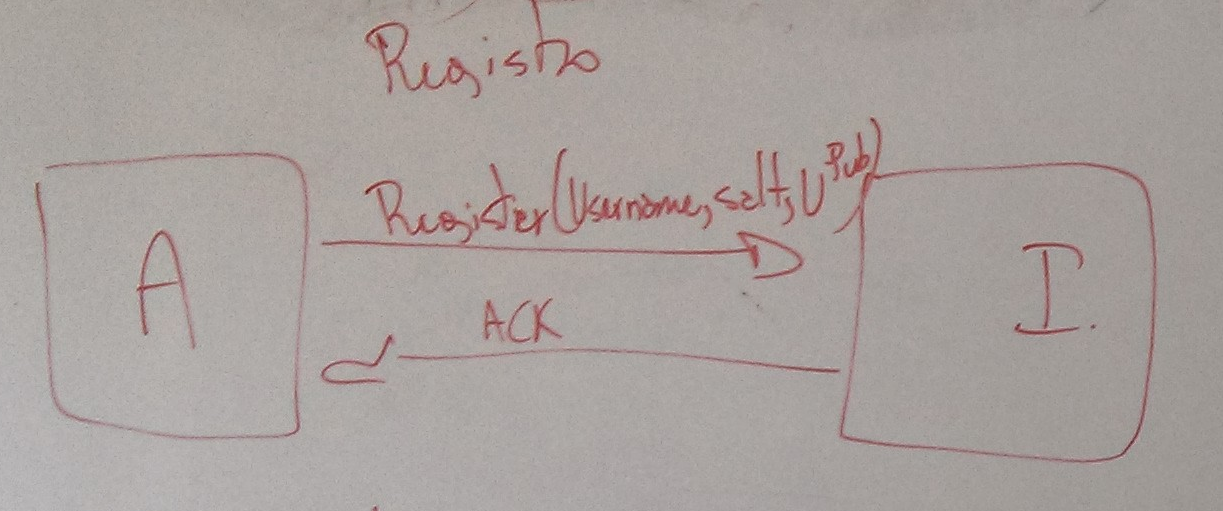
\includegraphics[width=14cm]{../img/registration_protocol_mockup.png}\\

To register a new user account ($U$), the node first
has to choose a \textit{username} and a \textit{password}.
%The \textit{username} should be unique in the network.
% The user checks if the username exists by sending a
% REGISTER(username, identity_file: [[c(user_keys_file), salt]).
% This operation use a accounted routing algorithm that uses only trusted
% nodes. When the register operation reaches the closest node to the username,
% it propagates a TRUSTSET_USERNAME_REGISTRATION operation. This operation sends a
% call to each node in the trustset of the node, which then pass to do a council
% meeting. If the meeting results in favor, each of them sends a
% OK_USERNAME_REGISTRATION(user_identity_file_name) to node doing the REGISTER operation.
% 
% DETAILS OF THE REGISTER OPERATION
% DETAILS OF THE COUNCIL MEETING --> Explain before, in trusted node part 
% 

% key store file
Then, a key derivation process is issued to generate the user Private and
Public Keys. The
key derivation utilizes a Salt ($U^{salt}$) and a Password ($U^{password}$) to
obtain the user's private and public Keys
($U^{priv}$ and $U^{pub}$).
The node  looks for the set $I$ set of nodes that will constitute the
identification service for the user $U$. To obtain the list of nodes that provides the user identification service for
the username $U^{username}$, the node $A$ computes its key $K$ such that $K =
SHA(U^{username})$. 

Then the node $A$ sends a request to every node $I_i$ in $I$ to register the
$U^{salt}$ and $U^{Pub}$ under the chosen  username  $U^{username}$.

Each node in $I$ agrees in generating a random challenge~\ref{sec:challenges_puzzles}, which is then sent to the
client $A$ by every node $I_i \in I$ using the node public key to encrypt the
message.

If the node $A$ succeeds in answering correctly to the challenge, each node $I_i \in I$ then sends a user registration confirmation message to all nodes
in $I$ containing the new user public key and salt. If a node $I_i$ receives at
least $\frac{L}{2} + 1$ identical user registration confirmation messages from
the others nodes in $I$, it sends a affirmative answer to the node $A$.

When the node
$A$ receives at least $\frac{L}{2} + 1$ identical affirmative answers from
$I$ regarding the user registration, then $A$ assumes that the user was
actually registered.

%unique username
In case that the username was taken,
the node $A$ is prompted for a new username.



\subsection{User private key recovery}
\label{sec:private_key_recovery}
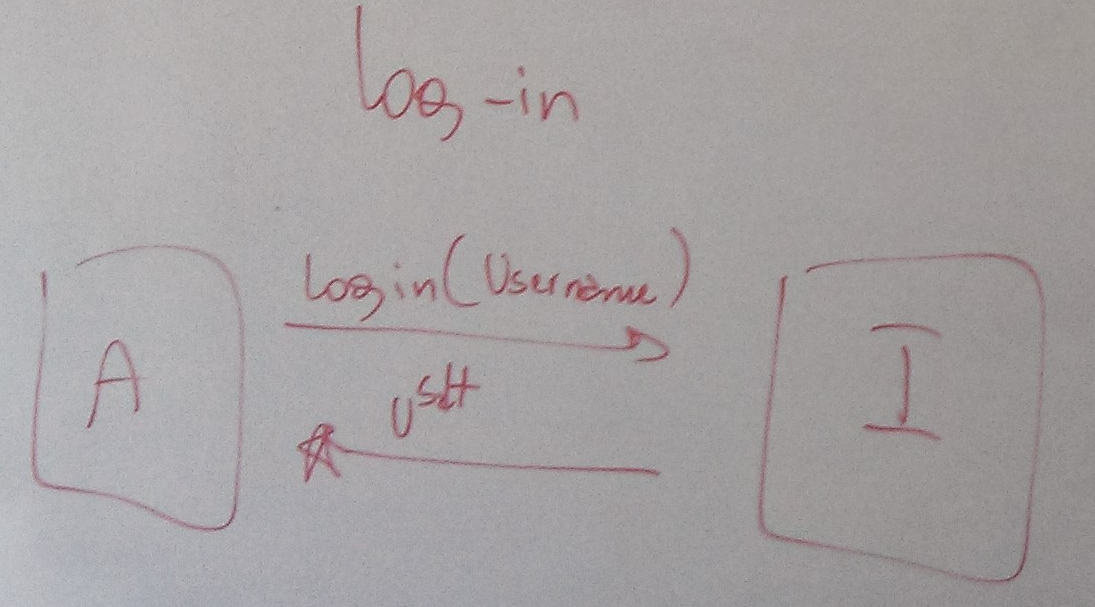
\includegraphics[width=14cm]{../img/login_protocol_mockup}\\

First, the node $A$ looks for the set $I$ set of nodes that will constitute the
identification service for the user $U$.
To obtain the list of nodes $I$ that provides the user identification service for
the username $U^{username}$, the node $A$ computes its key $K$ such that $K =
SHA(U^{username})$. 
Then the node $A$ sends a request to every node $I_i$ in $I$ to obtain the user
salt $U^{salt}$ needed to derive the user private key $U^{priv}$.
 When the node $A$ receives at least $\frac{L}{2} + 1$ identical affirmative answers from
$I$ regarding the user salt, then $A$ assumes that the salt retrieved
corresponds to the one registered previously by the user ($U^{salt}$). Finally,
the node proceeds to derive the user private key $U^{priv}$ using his user password $U^{password}$.

\subsection{User Sign-in}
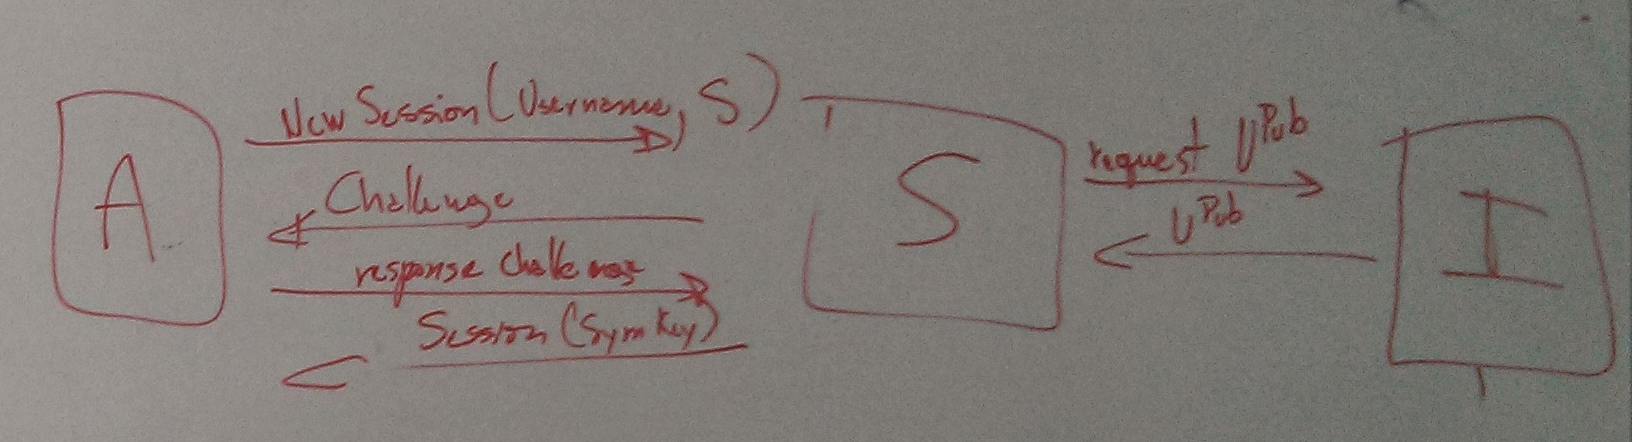
\includegraphics[width=14cm]{../img/session_creation_protocol_mockup}\\

Before carrying out a transaction for a client $A$, $S$ proceeds to
verify the identity of the client from another set $I$ of nodes. At the end of
the identification process, the objective is to return a session key to $A$
and to store the created session on the nodes that belong $S$.

Each node in $S$ agrees in generating a random challenge~\ref{sec:challenges_puzzles}, which is then sent to the
client $A$ by every node $S_i \in S$ using the user public key to encrypt the
message.

Then, client $A$ responds each request with the corresponding answer to the
challenge encrypted with his user private key $U^{priv}$, generating
$E^{challenge}_{U^{priv}}$. 

Upon reception of the $E^{secret_i}_{U^{priv}}$ message from the client $A$, every node in $S$
starts looking for the set $I$ of nodes that will constitute the quasi
identification authority. As seen in user identification service~\ref{sec:user_identificators}, to
determine which nodes belong to $I$, $S$ computes
its key $K$ such that $K = SHA(U^{username})$.

Then each node in $S$ sends a request to every node $I_i$ in $I$ asking for the Username public key $U^{pub}$. When a node
$S_i$ of $S$ receives at least $\frac{L}{2} + 1$ identical answers from
$I$ regarding the $U^{pub}$, then $S_i$ assumes that the public key received
actually corresponds to the Username being identified. Each node $S_i$ in $S$
uses the $U^{pub}$ to decrypt $E^{secret_i}_{U^{priv}}$. If the result matches
the shared random secret $S^{secret}_i$, $S_i$ recognizes the node $A$ as the
user $U$.
Lastly, each node in $S$ agrees in the generation of the sessions keys for the
node $A$, which is then sent to the client $A$ by every node $S_i \in S$ using
the user public key to encrypt it. The session keys are stored in the
nodes that belong to $S$.

\subsection{Logout}
The session are maintained by each service the user identified with. To close a
session, the node identified as the user $U$ sends a session close request to
the service $S$ using the session keys for the transaction. Also, the sessions
keys are issued for a certain time. After that time is passed, the node needs
to ask for a new session key with the service.


\subsection{Password Change}

First, the node $A$ needs to recover his actual private key using the process
in~\ref{sec:private_key_recovery}. Then the node $A$ generates a new private/public
key pair using the new password.  With this, the node $A$ request a
password change to every node $I_i$ in $I$. The request is signed with the
actual user private keys, and includes the new user public key $U^{pub}_{new}$
and salt used to derive his new private key $U^{salt}_{new}$. 
Each node $I_i \in I$ then sends a password change confirmation message to all nodes
in $I$ containing the new user public key and salt. If a node $I_i$ receives at
least $\frac{L}{2} + 1$ identical password change confirmation messages from
the others nodes in $I$, it sends a affirmative answer to the node $A$.
 When the node $A$ receives at least $\frac{L}{2} + 1$ identical affirmative
answers from $I$ regarding the user password change, then $A$ assumes that the
user keys (and password) were updated.



\chapter{Evaluation}
\label{sec:evaluation}
In this section we present a probability assessment of
the algorithms used in our quasi identification system, and show that it is highly
improbable to fail.

In this section, $p$ represents the probability that a single node is
malicious, and $N$ the total number of nodes in the DHT. We conduct every
assessment with two different values for $p$, being $p = 0.3$ and $p = 0.05$.
The former corresponds to the limit above which our relaxed version of the
byzantine agreement collapses. The latter corresponds to the value most
commonly found in the literature about malicious attacks in P2P
systems~\cite{p2p_certification}.
%, as well as a set of simulations and performance
%results.

%%%Theoretical evaluation

\section{Securing the nodes of a Leafset}
\label{sec:eval_leafset}
  
  \subsection{\textit{Probability of failure}}
  
  \begin{table}
    \centering
    \footnotesize
    \begin{tabular}{|c|c|c|}
      \cline{2-3}
      \multicolumn{1}{c|}{}&  \multicolumn{2}{c|}{\textbf{Probability to fail}} \\ \cline{2-3}
      \hline
      \textbf{Size of Trusted Set (L)} & \textbf{p = 0,3} & \textbf{p = 0,05} \\
      \hline \hline
      8 &  $0.0081$              & $6.25 \times 10^{-6}$  \\
      \hline
      16 & $6.56 \times 10^{-5}$ & $ 3.9 \times 10^{-11}$ \\
      \hline
      32 & $4.3 \times 10^{-9}$  & $ 1.52 \times 10^{-21} $  \\
      \hline
    \end{tabular}
    \caption{Probability of failure when securing a leafset}
    \label{tab:p_leafset}
  \end{table}
  
  Table~\eqref{tab:p_leafset} shows the probability of failure when securing the
  nodes of a leafset. The algorithm fails to get the leafset of a given node
  $K_{root}$ if $\frac{L}{2}$ consecutive nodes are malicious in a leafset. This
  probability is given by
  
  \begin{equation} \label{eq:p_leafset}
    P= p^{\frac{L}{2}}
  \end{equation}
  
  \subsection{\textit{Message complexity}}

      %As seen in~\cite{p2p_certification}
      According to the equation~\eqref{eq:p_leafset}, the probability of having
more than 4 consecutive malicious nodes when using the Diversity Trusted
Routing is around $6.25 \times 10^{-6}$. We can thus consider it highly
improbable that more than 4 routing attempts will be necessary  to secure a
leafset of a node near $K_{root}$. An upper bound of the cost to get the
leafset of $K_{root}$ is given by
      
      \begin{align} \label{eq:p_leafset}
        n &= \underbrace{O(log_{2b}(N)) + 4 \times O(log_{2b}(N))}_\text{First
and Diversity Routing} + \underbrace{Q+4}_\text{Direct IP} \\
        n &= 5 \times O(log_{2b}(N)) +  Q+4 
      \end{align}
      
      where $Q$ is the maximum number of tries to get a leafset from a node
that belongs to the leafset of $K_{root}$. The probability of not being able to
retrieve a leafset from a node that belongs to the leafset of $K_{root}$ after
$Q = 16$ tries for a leafset size $ L = 16$ is $1.52 \times 10^{-21} $. This is
highly improbable, so we can consider that $L/2 = 8$ is a reasonable upper
bound for $Q$. 
      In the best case, the cost is reduced to $n = O(log(N))$ when the root
node $K_{root}$ is honest. Thus, the message complexity of the chosen leafset
securing algorithm~\cite{p2p_certification} easily scales when the size of the
DHT increases.



%\section{Normal service request}
\label{sec:eval_service_request}
  \begin{table}
    \centering
    \footnotesize
    \begin{tabular}{|c|c|c|}
      \cline{2-3}
      \multicolumn{1}{c|}{}&  \multicolumn{2}{c|}{\textbf{Probability to fail}} \\ \cline{2-3}
      \hline
      \textbf{Size of Trusted Set (L)} & \textbf{p = 0.3} & \textbf{p = 0.05} \\
      \hline \hline
      8 &  $0.188$ & $6.64 \times 10^{-5}$ \\
      \hline
      16 & $0.079$ & $6.57 \times 10^{-8}$  \\
      \hline
      32 & $0.016$ & $8.24 \times 19^{-14}$  \\
      \hline
    \end{tabular}
    \caption{Probability of failure when doing a normal service request}
    \label{tab:p_service_request}
  \end{table}
  
  \begin{enumerate}
    \item{\textit{Probability of failure:}}
    The user registration between a node $A$ and $S$ can fail (a) if $S$does
not respond to $A$ during the registration request or during the registration
progress, or (b) if $S$ does not send the ACKs to $A$ to terminate the user
registration. In both cases, this corresponds to the probability that more than
$L/2$ nodes of $S$ are malicious. The probability of encountering exactly $k$
malicious nodes among $L +1$ is given by the binomial distribution

    \begin{equation}
      P_{K malicious} = \begin{pmatrix} L+1 \\ k\end{pmatrix} p^k (1-p)^{L+1-k}
    \end{equation}

    where $p$ is the probability that a single node is malicious. Hence the
probability of facing at most k malicious nodes is 

    \begin{equation}
      P_{\leq k} = \sum_{i=1}^{k} \begin{pmatrix} L+1 \\ k\end{pmatrix} p^i (1-p)^{L+1-i}
    \end{equation}

    Therefore, the probability of facing more than $k$ malicious nodes among
$n$ is given by

    \begin{equation}
      P_{\ge k} = P_{\leq n} - P_{\leq k}
    \end{equation}

    and the probability that $S$ will not respond is

    \begin{align}
      P_{\ge L/2} &= P_{\leq L+1} - P_{\leq L/2} \\
      &= \sum_{i=1}^{L+1} \begin{pmatrix} L+1 \\ i\end{pmatrix} p^i (1-p)^{L+1-i}
      - \sum_{i=1}^{L/2} \begin{pmatrix} L+1 \\ i\end{pmatrix} p^i (1-p)^{L+1-i}
    \end{align}

    %% TODO: figure with the likeliness of dealing with an increains gnumber k of malicious nodes among a leafset comprising 32 nodes.

    Then the probability that $S$ will not respond to the user registration
request or to not send the final ACKs is

    \begin{align}
      P_{AS} &= (1- P_{\ge L/2}) P_{\ge L/2} +  P_{\ge L/2} \\
      P_{AS} &= 2P_{\ge L/2}) + P^2_{\ge L/2}
    \end{align}


    Table~\eqref{tab:p_account_registration} shows the probability of failure
between $A$ and $S$, for a leafset size of $L = \{8,16,32\}$.

    
    \item{\textit{Message complexity:}}
    First, $A$ must get the leafset of $S$. The associated cost is $n = 5
\times O(log_{2b}(N)) + Q + 4$ (as seen in section~\ref{sec:eval_leafset}).
    The number $n$ of message inherent to the transaction itself is given by

    \begin{align}
      n &= \underbrace{2(L+1)}_\text{Init} \underbrace{r(L+1)}_\text{Data} \underbrace{L+1}_\text{ACKs}\\
      n &= (r+3)(L+1)
    \end{align}
    where $r$ corresponds to the number of data messages sent by $A$ to $S$,
and fully depends on the transaction. The total cost is then

    $$
      n_{total} = 5 \times O(log_{2b}(N)) + Q + 4 + (r+3)(L+1)
    $$    
    The total cost only depends on the size $L$ of the leafset, which is a
constant, and $O(log(N))$. In the best case, 

    $$
      n_{total} = O(log_{2b}(N)) + (r+3)(L+1)
    $$
    Therefore, the cost of a transaction between $A$ and service $S$ remains
scalable when the size $N$ of the DHT increases.

  \end{enumerate}


\section{Account registration}
\label{sec:eval_account_registration}
  % TODO Recalculate table
  \begin{table}
    \centering
    \footnotesize
    \begin{tabular}{|c|c|c|}
      \cline{2-3}
      \multicolumn{1}{c|}{}&  \multicolumn{2}{c|}{\textbf{Probability to fail}} \\ \cline{2-3}
      \hline
      \textbf{Size of Trusted Set (L)} & \textbf{p = 0.3} & \textbf{p = 0.05} \\
      \hline \hline
      %8 &  $0.0988087$ & $3.32222 \times 10^{-5}$ \\
      %\hline
      %16 & $0.0402769$ & $3.28714 \times 10^{-8}$  \\
      %\hline
      %32 & $0.00782066$ & $4.11893 \times 10^{-14}$  \\

      8 &  $0.098$ & $3.322 \times 10^{-5}$ \\
      \hline
      16 & $0.040$ & $3.287 \times 10^{-8}$  \\
      \hline
      32 & $0.007$ & $4.118 \times 10^{-14}$  \\
      \hline
    \end{tabular}
    \caption{Probability of failure when registering a new user account}
    \label{tab:p_account_registration}
  \end{table}
  
  \subsection{\textit{Probability of failure}}
    The user registration between a node $A$ and $I$ can fail if $I$ does
not respond (or responds false information) to $A$ during the registration request or during the registration
progress. In all cases, this corresponds to the probability that more than
$L/2$ nodes of $I$ are malicious. The probability of encountering exactly $k$
malicious nodes among $L +1$ is given by the binomial distribution

    \begin{equation} \label{eq:p_k_malicious_nodes}
      P_{K malicious} = \begin{pmatrix} L+1 \\ k\end{pmatrix} p^k (1-p)^{L+1-k}
    \end{equation}

    where $p$ is the probability that a single node is malicious. Hence the
probability of facing at most k malicious nodes is 

    \begin{equation}
      P_{\leq k} = \sum_{i=1}^{k} \begin{pmatrix} L+1 \\ k\end{pmatrix} p^i (1-p)^{L+1-i}
    \end{equation}

    Therefore, the probability of facing more than $k$ malicious nodes among
$n$ is given by

    \begin{equation} \label{eq:p_malicious_ge_k}
      P_{\ge k} = P_{\leq n} - P_{\leq k}
    \end{equation}

    and the probability that $I$ will not respond is

    %% for wolfram alpha
    %% P_{\leq L+1} =  sum( ((L+1) choose i)  * p^i * (1-p)^(L+1-i), from i=1 to L+1) where L=8, p=0.3
    %% P_{\ge L/2}  =  sum( ((L+1) choose i)  * p^i * (1-p)^(L+1-i), from i=1 to L+1) - sum( ((L+1) choose i)  * p^i * (1-p)^(L+1-i), from i=1 to L/2)  where L=8, p=0.3

    \begin{align} \label{eq:p_malicious_ge_L_2}
      P_{\ge L/2} &= P_{\leq L+1} - P_{\leq L/2} \\
      &= \sum_{i=1}^{L+1} \begin{pmatrix} L+1 \\ i\end{pmatrix} p^i (1-p)^{L+1-i}
      - \sum_{i=1}^{L/2} \begin{pmatrix} L+1 \\ i\end{pmatrix} p^i (1-p)^{L+1-i}
    \end{align}

    %% TODO: figure with the likeliness of dealing with an increains gnumber k of malicious nodes among a leafset comprising 32 nodes.

    Then the probability that $I$ will not respond to the user registration
request or responds with a fake registration response is

    \begin{align}
      P_{AI} &= P_{\ge L/2} 
    \end{align}


    Table~\eqref{tab:p_account_registration} shows the probability of failure
between $A$ and $I$, for a leafset size of $L = \{8,16,32\}$.

    
  \subsection{\textit{Message complexity}}
    First, $A$ must get the leafset of $I$. The associated cost is $n = 5
\times O(log_{2b}(N)) + Q + 4$ (as seen in section~\ref{sec:eval_leafset}).
    The number $n$ of message inherent to the transaction itself is given by

    \begin{align}
      n &= \underbrace{2(L+1)}_\text{Init} +
           \underbrace{L+1}_\text{Registration Data} +
           \underbrace{(L+1)L}_\text{I registration confirmations} +
           \underbrace{L+1}_\text{ACKs}\\
      n &= (L+4)(L+1)\\
      n &= L^2+ 5L + 4
    \end{align}

     The total cost is then
    $$
      n_{total} = 5 \times O(log_{2b}(N)) + Q + 4 + L^2 + 5L + 4
    $$    

    The total cost only depends on the size $L$ of the leafset, which is a
constant, and $O(log(N))$. In the best case, 
    $$
      n_{total} = O(log_{2b}(N)) + L^2 + 5L + 4
    $$
    Therefore, the cost of a transaction between $A$ and service $I$ remains
scalable when the size $N$ of the DHT increases.

\section{Lazy User's Information Store Maintenance}
\label{sec:eval_lazy_maintenance}

  \begin{table}
    \centering
    \footnotesize
    \begin{tabular}{|c|c|c|c|}
      \cline{3-4}
      \multicolumn{2}{c|}{} &  \multicolumn{2}{c|}{\textbf{Probability to fail}} \\ \cline{2-3}
      \cline{2-4}
      \multicolumn{1}{c|}{} & \textbf{L} & \textbf{p = 0.3} & \textbf{p = 0.05} \\
      \hline
      \multirow{3}{*}{\rotatebox[origin=c]{90}{\textbf{Case 1}}} & 8 &  &  \\
      \cline{2-4}
      \multicolumn{1}{|c|}{} & 16 &  &  \\
      \cline{2-4}
      \multicolumn{1}{|c|}{} & 32 &  &  \\
      \hline
      \multirow{3}{*}{\rotatebox[origin=c]{90}{\textbf{Case 2}}} & 8 &  &  \\
      \cline{2-4}
      \multicolumn{1}{|c|}{} & 16 &  &  \\
      \cline{2-4}
      \multicolumn{1}{|c|}{} & 32 &  &  \\
      \hline
    \end{tabular}
    \caption{Probability of failure when performing the user's information store maintenance}
    \label{tab:p_lazy_maintenance}
  \end{table}
  
  \subsection{\textit{Probability of failure}}

    We must consider two cases for certificate log maintenance: when a new node
enters the leafset (case 1) and when a node leaves the leafset (case 2).

    \paragraph{\textbf{Case 1}} A new node enters the leafset. The maintenance
of the user information fails if it encounters $\frac{L}{2}$ consecutive
malicious nodes when building the node interval to retrieve the logs, or if
more than $\frac{L}{2}$ nodes are malicious (impossibility to have more than
$\frac{L}{2} +1$ identical answers).\\
    The probability $P_1$ of having $\frac{L}{2}$ consecutive malicious nodes
is given by equation~\ref{eq:p_k_malicious_nodes}: $P_1 = p^{L/2}$, and the
probability $P_2$ of not being able to retrieve at least $\frac{L}{2} +1$
identical answers is given by equation~\ref{eq:p_malicious_ge_L_2}: $P_2 =
P_{\ge L/2}$.\\
 Hence the total probability that this maintenance operation will
fail is

$$
  P_{total} = P_1 + (1-P_1) P_2
$$


    \paragraph{\textbf{Case 2}} A node is leaving the leafset. The user
information cannot be repaired if the node cannot repair its leafset (adding a
node on the left or right side), or if it is impossible to find at least
$\frac{L}{2} +1$ identical answers to retrieve the user information.

A node cannot repair its leafset if $\frac{L}{2} -1$ consecutive nodes are
malicious with a probability $P_1 = p^{L/2 - 1}$ and the user information
retrieval fails with a probability $P_2 = P_{\ge L/2}$.\\
Hence the total probability of failure is
$$
  P_{total} = P_1 + (1-P_1)P_2
$$

Table~\ref{tab:p_lazy_maintenance} computes the probability that a maintenance
operation will fail, given increasing leafset sizes $L = {8,16,32}$.


\section{User private key recovery}
\label{sec:eval_private_key_recovery}
% TODO Recalculate table
  \begin{table}
    \centering
    \footnotesize
    \begin{tabular}{|c|c|c|}
      \cline{2-3}
      \multicolumn{1}{c|}{}&  \multicolumn{2}{c|}{\textbf{Probability to fail}} \\ \cline{2-3}
      \hline
      \textbf{Size of Trusted Set (L)} & \textbf{p = 0.3} & \textbf{p = 0.05} \\
      \hline \hline
      8 &  $0.098$ & $3.322 \times 10^{-5}$ \\
      \hline
      16 & $0.040$ & $3.287 \times 10^{-8}$  \\
      \hline
      32 & $0.007$ & $4.118 \times 10^{-14}$  \\
      \hline
    \end{tabular}
    \caption{Probability of failure when recovering user private key}
    \label{tab:p_private_key_recovery}
  \end{table}

  \subsection{\textit{Probability of failure}}

    The user private key recovery between a node $A$ and $I$ can fail (a) if $I$ does
not respond (or responds fake information) to $A$ during the key recovery
request. While a response with fake information (like a salt forged by malicious nodes) can be more dangerous for the
user, the probability remains the same, corresponding to the
probability that more than $L/2$ nodes of $I$ are malicious.\\
    The probability that $I$ will not respond to the user private key recovery
request (or that $I$ responds fake user information) is the probability of
facing more than $\frac{L}{2} +1$ malicious nodes in $I$. This probability is given by the
equation~\ref{eq:p_malicious_ge_L_2} and hence the probability that the user
private key recovery fails is:

\begin{equation} \label{eq:L_2_malicious_A_I}
 P_{AI} = P_{\ge L/2}
\end{equation}

    Table~\eqref{tab:p_private_key_recovery} shows the probability of failure
between $A$ and $I$, for a leafset size of $L = \{8,16,32\}$.

    
  \subsection{\textit{Message complexity}}
    First, $A$ must get the leafset of $I$. The associated cost is $n = 5
\times O(log_{2b}(N)) + Q + 4$ (as seen in section~\ref{sec:eval_leafset}).
    The number $n$ of message inherent to the transaction itself is given by

    \begin{align}
      n &= \underbrace{2(L+1)}_\text{Init} + \underbrace{L+1}_\text{Data} +  \underbrace{L+1}_\text{ACKs}\\
      n &= 4(L+1)
    \end{align}
     The total cost is then

    $$
      n_{total} = 5 \times O(log_{2b}(N)) + Q + 4 + 4(L+1)
    $$    
    The total cost only depends on the size $L$ of the leafset, which is a
constant, and $O(log(N))$. In the best case, 

    $$
      n_{total} = O(log_{2b}(N)) + 4(L+1)
    $$
    Therefore, the cost of a transaction between $A$ and service $I$ remains
scalable when the size $N$ of the DHT increases.


\section{User Sign-in}
\label{sec:eval_sign_in}
  \begin{table}
    \centering
    \footnotesize
    \begin{tabular}{|c|c|c|}
      \cline{2-3}
      \multicolumn{1}{c|}{}&  \multicolumn{2}{c|}{\textbf{Probability to fail}} \\ \cline{2-3}
      \hline
      \textbf{Size of Trusted Set (L)} & \textbf{p = 0.3} & \textbf{p = 0.05} \\
      \hline \hline
      8 &  $0.188$ & $6.64 \times 10^{-5}$ \\
      \hline
      16 & $0.079$ & $6.57 \times 10^{-8}$  \\
      \hline
      32 & $0.016$ & $8.24 \times 10^{-14}$  \\
      \hline
    \end{tabular}
    \caption{Probability of failure in user sign-in}
    \label{tab:p_sign_in}
  \end{table}
  
  \subsection{\textit{Probability of failure}}
    A sign-in request between a node $A$ and the service $S$, can fail (a) if the identification service $I$ does
not respond (or responds fake information) to $S$ during the user information recovery
request, or (b) if $S$ does not respond (or responds fake information) to $A$
during the challenge or the session keys generation. While a response with fake information can be more dangerous for the
user, the probability remains the same, corresponding to the
probability that more than $L/2$ nodes of $I$ (or $S$) are malicious. The probability of
encountering exactly $k$ malicious nodes among $L +1$ is given by the binomial
distribution

    \begin{equation}
      P_{K malicious} = \begin{pmatrix} L+1 \\ k\end{pmatrix} p^k (1-p)^{L+1-k}
    \end{equation}

    where $p$ is the probability that a single node is malicious. Hence the
probability of facing at most k malicious nodes is 

    \begin{equation}
      P_{\leq k} = \sum_{i=1}^{k} \begin{pmatrix} L+1 \\ k\end{pmatrix} p^i (1-p)^{L+1-i}
    \end{equation}

    Therefore, the probability of facing more than $k$ malicious nodes among
$n$ is given by

    \begin{equation}
      P_{\ge k} = P_{\leq n} - P_{\leq k}
    \end{equation}

    and the probability that $I$/$S$ will not respond is

    \begin{align}
      P_{\ge L/2} &= P_{\leq L+1} - P_{\leq L/2} \\
      &= \sum_{i=1}^{L+1} \begin{pmatrix} L+1 \\ i\end{pmatrix} p^i (1-p)^{L+1-i}
      - \sum_{i=1}^{L/2} \begin{pmatrix} L+1 \\ i\end{pmatrix} p^i (1-p)^{L+1-i}
    \end{align}

    %% TODO: figure with the likeliness of dealing with an increains gnumber k of malicious nodes among a leafset comprising 32 nodes.

    Then the probability that $I$ will not respond to the service user
information recovery request, or that $S$ not respond to the node $A$ is

    \begin{align}
      P_{AI} &= (1- P_{\ge L/2}) P_{\ge L/2} +  P_{\ge L/2} \\
      P_{AI} &= 2P_{\ge L/2} - P^2_{\ge L/2}
    \end{align}


    Table~\eqref{tab:p_sign_in} shows the probability of failure
between $A$, the service $S$ and $I$, for a leafset size of $L = \{8,16,32\}$.

  \subsection{\textit{Message complexity}}
    First, $A$ must get the leafset of $S$. The associated cost is $n = 5
\times O(log_{2b}(N)) + Q + 4$ (as seen in section~\ref{sec:eval_leafset}).
Then, every node in $S$ must get the leafset of $I$, with each leafset request
having the same associated cost as before $n = (L+1)(5 \times O(log_{2b}(N)) + Q + 4)$~\ref{sec:eval_leafset}.
    The number $n$ of message inherent to the transaction itself is given by

    \begin{align}
      % TODO: + ommited for space, fix this with other way to express this
      n &= \underbrace{2(L+1)}_\text{Init A with S} +
           \underbrace{2(L+1)^2}_\text{Init S with I} +
           \underbrace{(L+1)^2}_\text{Data from I to S} +
           \underbrace{(L+1)L}_\text{Init Challenge} +
           \underbrace{2(L+1)}_\text{S challenges A} +
           \underbrace{L+1}_\text{ACKs}\\
      n &= 5(L+1) + 3(L+1)(L+1)+ (L+1)L\\
      n &= 4L^2 +12L + 8 
    \end{align}
     The total cost is then

    $$
      n_{total} = (L +2)(5 \times O(log_{2b}(N)) + Q + 4) + 4L^2 +12L + 8 
    $$    
    The total cost only depends on the size $L$ of the leafset, which is a
constant, and $O(log(N))$. In the best case, 

    $$
      n_{total} = (L +2)O(log_{2b}(N)) + 4L^2 +12L + 8 
    $$
    Therefore, the cost of a transaction between $A$ and service $I$ remains
scalable when the size $N$ of the DHT increases.

\section{Logout}
  \label{sec:eval_logout}
  \begin{table}
    \centering
    \footnotesize
    \begin{tabular}{|c|c|c|}
      \cline{2-3}
      \multicolumn{1}{c|}{}&  \multicolumn{2}{c|}{\textbf{Probability to fail}} \\ \cline{2-3}
      \hline
      \textbf{Size of Trusted Set (L)} & \textbf{p = 0.3} & \textbf{p = 0.05} \\
      \hline \hline
      8 &  $0.098$ & $3.322 \times 10^{-5}$ \\
      \hline
      16 & $0.040$ & $3.287 \times 10^{-8}$  \\
      \hline
      32 & $0.007$ & $4.118 \times 10^{-14}$  \\
      \hline
    \end{tabular}
    \caption{Probability of failure in user logout}
    \label{tab:p_logout}
  \end{table}
  
  \subsection{\textit{Probability of failure}}
    The user logout between a node $A$ and $S$ can fail if $S$ does
not respond (or responds false information) to $A$ during the logout request.
  In all cases, this corresponds to the probability that more than
$L/2$ nodes of $I$ are malicious. The probability of encountering exactly $k$
malicious nodes among $L +1$ is given by the binomial distribution

    \begin{equation}
      P_{K malicious} = \begin{pmatrix} L+1 \\ k\end{pmatrix} p^k (1-p)^{L+1-k}
    \end{equation}

    where $p$ is the probability that a single node is malicious. Hence the
probability of facing at most k malicious nodes is 

    \begin{equation}
      P_{\leq k} = \sum_{i=1}^{k} \begin{pmatrix} L+1 \\ k\end{pmatrix} p^i (1-p)^{L+1-i}
    \end{equation}

    Therefore, the probability of facing more than $k$ malicious nodes among
$n$ is given by

    \begin{equation}
      P_{\ge k} = P_{\leq n} - P_{\leq k}
    \end{equation}

    and the probability that $S$ will not respond is

    \begin{align}
      P_{\ge L/2} &= P_{\leq L+1} - P_{\leq L/2} \\
      &= \sum_{i=1}^{L+1} \begin{pmatrix} L+1 \\ i\end{pmatrix} p^i (1-p)^{L+1-i}
      - \sum_{i=1}^{L/2} \begin{pmatrix} L+1 \\ i\end{pmatrix} p^i (1-p)^{L+1-i}
    \end{align}

    %% TODO: figure with the likeliness of dealing with an increains gnumber k of malicious nodes among a leafset comprising 32 nodes.

    Then the probability that $S$ will not respond to the user logout 
request or responds with a fake logout response is

    \begin{align}
      P_{AI} &= P_{\ge L/2} 
    \end{align}


    Table~\eqref{tab:p_logout} shows the probability of failure
between $A$ and $S$, for a leafset size of $L = \{8,16,32\}$.

    
  \subsection{\textit{Message complexity}}
    First, $A$ must get the leafset of $S$. The associated cost is $n = 5
\times O(log_{2b}(N)) + Q + 4$ (as seen in section~\ref{sec:eval_leafset}).
    The number $n$ of message inherent to the transaction itself is given by

    \begin{align}
      n &= \underbrace{2(L+1)}_\text{Init} +  \underbrace{L+1}_\text{Logout Request} + \underbrace{L+1}_\text{ACKs}\\
      n &= 4(L+1)
    \end{align}
     The total cost is then

    $$
      n_{total} = 5 \times O(log_{2b}(N)) + Q + 4 + 4(L+1)
    $$    
    The total cost only depends on the size $L$ of the leafset, which is a
constant, and $O(log(N))$. In the best case, 

    $$
      n_{total} = O(log_{2b}(N)) + 4(L+1)
    $$
    Therefore, the cost of a transaction between $A$ and service $I$ remains
scalable when the size $N$ of the DHT increases.

\section{Password Change}
  \label{sec:eval_password_change}
  \begin{table}
    \centering
    \footnotesize
    \begin{tabular}{|c|c|c|}
      \cline{2-3}
      \multicolumn{1}{c|}{}&  \multicolumn{2}{c|}{\textbf{Probability to fail}} \\ \cline{2-3}
      \hline
      \textbf{Size of Trusted Set (L)} & \textbf{p = 0.3} & \textbf{p = 0.05} \\
      \hline \hline
      8 &  $0.098$ & $3.322 \times 10^{-5}$ \\
      \hline
      16 & $0.040$ & $3.287 \times 10^{-8}$  \\
      \hline
      32 & $0.007$ & $4.118 \times 10^{-14}$  \\
      \hline
    \end{tabular}
    \caption{Probability of failure when changing the user password}
    \label{tab:p_password_change}
  \end{table}
  
  \subsection{\textit{Probability of failure}}
    A password change request between a node $A$, the identification service
$I$ can fail (a) if $L/2 + 1$ nodes in $I$ does not responds (or responds fake
information) correctly the password change confirmation message to the nodes 
$I_i \in I$ during the password change request, or (b) if $S$ does not respond (or responds fake information) to $A$
during the password change request. While a response with fake information can be more dangerous for the
user, the event of that happening is the same as when there is no response:
when more than $L/2$ nodes of $I$ are malicious.

%%%%%%%%%%%%% REPEATED PROBABILITY MESSAGE %%%%%%%%%%%%
The probability of encountering exactly $k$ malicious nodes among $L +1$ is given by the binomial
distribution

    \begin{equation}
      P_{K malicious} = \begin{pmatrix} L+1 \\ k\end{pmatrix} p^k (1-p)^{L+1-k}
    \end{equation}

    where $p$ is the probability that a single node is malicious. Hence the
probability of facing at most k malicious nodes is 

    \begin{equation}
      P_{\leq k} = \sum_{i=1}^{k} \begin{pmatrix} L+1 \\ k\end{pmatrix} p^i (1-p)^{L+1-i}
    \end{equation}

    Therefore, the probability of facing more than $k$ malicious nodes among
$n$ is given by

    \begin{equation}
      P_{\ge k} = P_{\leq n} - P_{\leq k}
    \end{equation}

    and the probability that $I$ will not respond is

    \begin{align}
      P_{\ge L/2} &= P_{\leq L+1} - P_{\leq L/2} \\
      &= \sum_{i=1}^{L+1} \begin{pmatrix} L+1 \\ i\end{pmatrix} p^i (1-p)^{L+1-i}
      - \sum_{i=1}^{L/2} \begin{pmatrix} L+1 \\ i\end{pmatrix} p^i (1-p)^{L+1-i}
    \end{align}
%%%%%%%%%%%%% REPEATED PROBABILITY MESSAGE %%%%%%%%%%%%

    %% TODO: figure with the likeliness of dealing with an increains gnumber k of malicious nodes among a leafset comprising 32 nodes.

    Then the probability that $I$ will not respond to the service user
information recovery request is

    \begin{align}
      P_{AI} &= P_{\ge L/2} \\
    \end{align}


    Table~\eqref{tab:p_password_change} shows the probability of failure
between $A$, the service $S$ and $I$, for a leafset size of $L = \{8,16,32\}$.

  \subsection{\textit{Message complexity}}
    First, $A$ must get the leafset of $I$. The associated cost is $n = 5
\times O(log_{2b}(N)) + Q + 4$ (as seen in section~\ref{sec:eval_leafset}).
%%% not needed, this has to be done in the leafset maintenance
%Then, every node in $I$ must get the leafset of $I$, with each leafset request
%having the same associated cost as before $n = (L+1)(5 \times O(log_{2b}(N)) + Q + 4)$~\ref{sec:eval_leafset}.
    The number $n$ of message inherent to the transaction itself is given by

    \begin{align}
      n &= \underbrace{2(L+1)}_\text{Init A with I} +
           \underbrace{(L+1)L}_\text{Data from I to I} +
           \underbrace{L+1}_\text{ACKs}\\
      n &= 3(L+1) + L(L+1)\\
      n &= L^2 + 4L + 3
    \end{align}
     The total cost is then

    $$
      n_{total} = 5 \times O(log_{2b}(N)) + Q + 4 +  L^2 + 4L + 3
    $$    
    The total cost only depends on the size $L$ of the leafset, which is a
constant, and $O(log(N))$. In the best case, 

    $$
      n_{total} = O(log_{2b}(N)) + L^2 + 4L + 3
    $$
    Therefore, the cost of a transaction between $A$ and service $I$ remains
scalable when the size $N$ of the DHT increases.

%We suppose in the following that the underlying
%reputation system makes an error $\varepsilon$ when classifying a
%node $X$ with a reputation $R(x) \geq \rho$, where $\rho \in [ 0 \cdots 1 ]$,
%and $ \varepsilon = f ( \rho )$. In other words, classifying a node $X$ as
%honest because its reputation is greater than $\rho$ has a
%probability of error $\varepsilon$.
%Let $n$ be the size of the Trusted Ring. The probability
%to have $k$ misclassified nodes in the Trusted Ring, that
%is $k$ malicious nodes is:
%
%$$
%P_{k_{malicious}} = \left(\!
%                          \begin{array}{c}
%                            n\\
%                            k
%                          \end{array}
%                    \!\right)              
%                    \varepsilon^{n-k} ( 1 - \varepsilon )^k
%$$
%
%Then, the probability to have at most $k$ malicious
%nodes in a Trusted Ring of size $n$ is:
%
%$$
%P_{\leq k} = \sum^{k}_{i=1} \left(\!
%                                \begin{array}{c}
%                                    n\\
%                                    k
%                                  \end{array}
%                            \!\right)              
%                    \varepsilon^{n-i} ( 1 - \varepsilon )^i
%$$
%
%Therefore, the probability to have $k$ or more malicious
%nodes in a Trusted Ring of size $n$ is:
%
%$$
%P_{\leq k} = \sum^{n}_{i=k} \left(\!
%                                \begin{array}{c}
%                                    n\\
%                                    i
%                                  \end{array}
%                            \!\right)              
%                    \varepsilon^{n-i} ( 1 - \varepsilon )^i
%$$
%
%The user identification fails when:
%\begin{enumerate}
%  \item The user cannot retrieve his own PKI from the \textit{trustset}.
%  \item or when the public key of the user fails to be retrieved.
%\end{enumerate}
%
%These failures can happen when the \textit{trustsets} storing the PKI or the public
%key have more malicious nodes than normal nodes.
%
%The probability that a \textit{trustset} has half or more malicious nodes, assuming a maximum
%classification error for the underlying reputation system
%of $5\%$, is .% FILL HERE
%%Hence the probability for having a fully erroneous trustset is theoretically possible, but
%%practically infeasible.
%
%Considering a maximum error rate of $5\%$ is a typical
%value for a reputation system. In some cases it may be
%over-estimated (for more details, please refer the results
%obtained for the WTR reputation system\cite{wrt_reputation_system}). This
%error hardly depends on the total number of malicious
%nodes in the network, and decreases when the ratio
%of malicious node decreases. The less malicious nodes
%there are in the system, the easier it is to discriminate
%against them.


\chapter{Validation and further discussion}
\label{sec:validation}
In this chapter we will discuss some security issues and the portability of our
solution.% and our decision about not having a password recovery mechanism

\section{System validation}

In comparison with centralized approaches, we know that the reliability of a
centralized identification service depends mostly on the
supporting host: its availability, its security and its capacity  to handle
significant amounts of concurrent requests. 
In practice this entails that a centralized identification service is not
foolproof: it is as trustworthy as the group of servers it runs on.
Well-established centralized identification services have been breached. %%%%%%%%% TODO: ADD REFERENCES
In a decentralized approach, the main issue is that the supporting hosts are
not accountable for their decisions and therefore cannot be trusted.\\

Because of this, as other P2P systems, a 100\% secure implementation cannot be achieved
(section~\ref{sec:pseudo-secure}).
%  Is the system valid?  fue demostrada la hipotesis?
Taking that into account, the goal of our approach was to drastically reduce the probability of a
malicious node impersonating another user who is using the identification
system. This was done using of a reputation system and trusted node management
to mitigate the effectivity of malicious nodes on identity usurpation attacks.

%% Then... the hypotesis was valid or not?
% cual es la peor probabilidad del sistema?
Our analysis shows that the highest probability of a protocol failing without using trusted nodes is 
with $L=8$, $p = 0.188$, and that the highest probability of a protocol failing
using trusted nodes is with $L=8$, $p = 6.64 \times 10^{-5}$. With $L=32$ the probabilities seems better, but without the use
of a trustset the probabilities remain at $p = 0.016$, too high to be usable in
reality. That is because in a system with $1000000$ users, with the probability
of a protocol failure being $p = 0.016$,  $16000$ of the users will have problems with
the protocols of the system. Then, a solution without the use of trusted nodes
is not acceptable with values of $L <= 32$. In comparison, using
only trusted nodes with $L=32$ we obtain a probability of $p =8.24 \times
10^{-14}$, meaning that in a system with $1000000$ users,
only $0.00000000824$ would fail.
% es aceptable o no? 
Then, using the trusted nodes for the system protocols we can be sure that failures in the
system's identification protocols are very unlikely to happen, being a valid
solution for solving the problem at hand.
% las probabilidades y evaluaciones ahcen el sistema valido o no?...IS VALID OR NOT??
With that, we can conclude that present solution is acceptable to be
used in real life applications.


% Al aumentar L, aumenta la cantidad de mensajes (n^2), es aceptable?
%% La cantidad de mensajes enviados durante los protocolos de registro de
%% usuario y de inicio de sesión depende en gran parte del valor de $L$.
%%  ....
If we analyze the message overhead of our protocols, we find that many depends
greatly in the value of $L$. $L$ is a fixed in the network and is
independent of the network size, so we can conclude that the messages costs
remains scalable with an message overhead of the order of $O(log(N))$.
 Still, high values of $L$ can generate a very high constant message cost. For that reason, the leafset size
$L$ should not be higher than $48$.  The implementation of a real life system
should take into consideration the amount of messages sent over the network
during an user session, as the high cost of our protocols, like the user
registration protocol and sign in protocol, can be justified when they represent just a
small fraction of all the system messages.

% cual seria el valor de L?
So, with our solution, with a leafset size of $L = 32$ nodes and a
$5\%$ proportion of malicious nodes distributed uniformly in the P2P system, the resulting probability of a false
positive, where a decision made by malicious nodes is adopted, is of the order
of $10^{-14}$. 
This value is far lower than any we have encountered in the
literature about decentralized identification systems. Also the system
maintains a cost scalable when the size of nodes $N$ of the DHT
increases. In terms of communications overhead, there is a trade off between its
cost and the security provided by the protocols. Using values of
$L = 16$ reduces the message overhead in the system and still provides a decent
probability of error of order $10^{-8}$, which in systems with a low presence of
malicious node can be acceptable. Then, if priority of the system is its
security and the message cost of the protocols is not
an issue for the system that will use it, a value of $L = 32$ is highly recommended. 


\section{Portability}

%% DHT -> Chord u otro?
Although our implementation relies on Pastry as its DHT, our approach can rely
on other building block implementations. For example, it is very simple to
switch the underlying DHT from Pastry to Chord, as Chord maintains structures
that are equivalent to the leafset and the routing table in Pastry, like using
the $r$ successors of Chord instead of the leafset of Pastry.

%% WTR -> Por otro? que valores necesita?
Our implementation can be built over any trust management service that
provides a way to find trusted nodes based on a reputation system
that provides a value $R(X)$, the value that represents the probability of a node
$X$ being honest, and maintains the structural properties of the underling
DHT. For example, WTR~\cite{bonnaire2009wtr} and
PeerTrust~\cite{xiong2004peertrust} are reputation systems that fulfill our
system requirements.

%system with the same properties explained
%in Section~\ref{sec:building_blocks}  is also required, but can be easily
%supported by any type of DHT, as long as it provides some type of key lookup
%service and.
%% CORPS -> explicar por que se usa la probabilidad 0,3 y 0,... en la parte de evaluacion


\section{Security issues}
%Regarding P2P networks and identification systems, there are many issues that
%hand that need to be accounted for when building the system. 

\subsection{Sybil attacks}
\label{sec:sybil_attacks}

The Sybil attack~\cite{the_sybil_attack} is a major concern if obtaining
network identities is cheap (NodeIDs). Such an attack allows to tampers with the ratio of
malicious nodes in the system as a single node acts under multiple identities:
the ratio can rise above the $30\%$ upper threshold. \\

A common feature of the Sybil attack is a single malicious user creating 
several identities with numerically close nodeIDs to be able to control a
substantial part of the DHT. We assume that the generation of the nodeIDs can
be verified by any node in the network, for instance the bootstrapping node or
the node with the closest nodeID. Our proposition assumes that nodeIDs are
computed from a public key and generated with a well-known public/private key
algorithm. We also suppose that the number of bits of these keys is sufficient
to avoid a brute force attack to reverse the SHA-1 function. During the
procedure to join the DHT, a node $A$ must provide several pieces of information to
the verifier node $X$: its public key $key_{pub}$, and the associated nodeID
are computed using
$nodeID = SHA1(key_{pub})$. $X$ can easily verify the correctness of the nodeID
with the public key. If they do not match, then $X$ prevents $A$ from joining
the ring.\\

Due to the mathematical properties of the SHA-1 hash function, it is
improbable that a node will find two keys $key_{pub1}$ and
$key_{pub2}$ such that $SHA1(key_{pub1}) = SHA1(key_{pub2})$. Therefore, it is
also doubtful that a node will find several public keys that give
numerically close nodeIDs in the ring. Thus, it is nearly impossible for a
node to control a substantial sector of the ring.\\

However, a single node can still generate several nodeIDs distributed over the
ring. This kind of Sybil attack does not allow a node to control a sector of the ring,
but it will increase failures in the DHT (routing failures, etc.).  Reputation
systems can efficiently mitigate Sybil attacks, but will collapse if the
ratio of malicious nodes is too high ($> 30\%$). To our knowledge, no existing reputation system can control a large
number of Sybil attacks in a DHT. For this reason, this is still a much
discussed topic within
the P2P research community.\\

As seen before in section~\ref{sec:challenges_puzzles}, other solutions to
mitigate the presence of Sybils is to make obtaining nodeIDs
exponentially difficult when a node needs a new
one. Existing solutions usually
rely on a set of servers to provide the nodeIDs, and are therefore not very
scalable.\\

The impact of a Sybil attack over the trusted ring of the reputation system
would mainly be at the level of its \textit{trustsets}. The main idea is to be
able to control various nodeIDs in a \textit{trustset}. This is not an easy
task: as shown above it is unfeasible to obtain numerically close
nodeIDs that belong to the same \textit{trustset}. Moreover, controlling a very
large number of trustsets is practically impossible, as it will require 
control of a very large number of nodeIDs. This is unfeasible due to the number of
transactions required from an attacker in order to establish a good reputation
for all of its nodeIDs, and then insert them into the Trusted
Ring~\cite{rosas2011corps}.\\

Analog to the problem of Sybil attacks to control multiple nodeIDs, an attacker
would likely try to control a large amount of user accounts in the
identification system. Having registered a large amount of usernames, a new
user could have difficulties in finding an unused username when registering in the
network. Also, having a large amount of identities through the services in the
network can be used to exploit some of their functionalities.
In our solution, we use computational challenges to mitigate the problem of a
node registering multiple users with the system. Another solution to
this problem is the use of CAPTCHA~\cite{von2003captcha} as an additional
challenge for user registration. While this type of challenge is not
without faults, it adds an additional layer of security against Sybil attacks.


\subsection{Collusion of nodes}

A collusion of nodes consists of an agreement made between various nodes to make
a combined attack, like the nodes of the reputation system colluding to artificially increase or decrease the reputation of a
set of nodes. Some existing
reputation systems, like WTR, can efficiently mitigate the effect of this kind
of attack. However, colluding nodes are able to sustain the attack
permanently in order to maintain a good reputation and remain in the trusted ring.
This will have a significant cost for the attackers, and for them to being able to manage a
great number of nodes in the trusted ring is very unlikely. 

\subsection{Offline attacks}
As our solution relies on a public/private key scheme to identify the user,
using derived keys from a public salt stored in the network a malicious node
could try to guess the password of a user. If the function used to derive the
private key has a low computation cost, a brute force attack that tries
different passwords and tests the derived private key with the user public key
can succeed if the attacker has the computational resources to do so. We
assumed that the key derivation function (e.g., bcrypt) is slow enough to make
it unfeasible for a computer to guess a user password in a reasonable 
amount of time. (more than 20 years)

\subsection{Passwords}
The traditional view is that passwords should be replaced by some better
mechanism, but despite significant research efforts into dislodging passwords,
they are still by far the most common authentication mechanism today.
Reasons for their prevalence include simplicity, price, and very strong user
familiarity.
It is known that the average user tends to use the
same password in more than one service, presenting serious security problems
for user identity integrity. A definitive solution to this problem has not
been found yet, but a strict password creation policy can mitigate this
problem. At the same time, this can also increase cases of forgotten passwords.

%\section{Password recovery}
%While the system does not allow password recovery operations...



%there can a time
%when the group nodes cannot decide over something in common, with the
%When commiting a transaction that needs a group of $n$ nodes
%
%
%This causes that after a transaction that
%involves a group of nodes, there is some amount of time where the nodes are not
%syncronized.

\subsection{Node data inconsistency}
Synchronization between nodes does not happen instantly. Also, thanks to
the different routes used in the network, simultaneous messages can reach a
destination at different times. So, as opposed to centralized systems, P2P
networks have certain times when the data in some nodes are inconsistent.
This is relevant for functions that need a
group of nodes to be synchronized at a certain time, because this ``temporal
inconsistency''  can cause fake positives or fake negatives in the protocols of
the network. For example, after a successful password change request, there can
be a time when some nodes will have the old user information. If another
request involving the user credentials is issued before these nodes have
synchronized their data, depending on what nodes are used in the request, the
validation that needs $\frac{L+1}{2}$ identical answers can fail or succeed.
While the timeframe when the nodes have not undergone synchronization is small,
it can still lead to problems if it is not considered in a protocol's
construction. In consequence, an added time span is considered for the
successful completion of the user registration and password change operations.

%To mitigate this problem, we propose the use of an active user information store
%maitenance.  and add consider a timespan of 1 to 2 seconds  




\chapter{Conclusion}
\label{sec:conclusion}
The main objective of this work was to propose a viable and secure
username/password based user identification scheme in structured P2P
networks using secure routing and building of trust between nodes.
With that in mind, we presented a quasi-identification service built on top of a DHT. It
replicates the user information needed to maintain the identification system
over multiple peers and retains identical results from a qualified majority to
certify that user public information corresponds to the correct registered user.
As in other P2P
systems, a 100\% secure implementation cannot be achieved
(section~\ref{sec:pseudo-secure}). Still, as seen in the
protocols evaluation (section~\ref{sec:evaluation}), an acceptable probability of error on the order
of $10^{-14}$ can be achieved with a leafset size of $L = 32$. Also, the system
maintains a scalable cost when the size of nodes $N$ in the DHT increases.
This was possible thanks to the use of a reputation system and trusted
nodes management, which mitigated the effectiveness of malicious node attacks in
the network.
An over DHT implementation makes the system portable for the most commonly used P2P networks.\\


%We are currently working on developing an identification service that
%allows password recovery operations while not compromising user identity
%through the integration of scalable trust mechanisms.

%\textbf{Acknowledgements.} The work presented was partially funded by a CONICYT scholarship.

\section{Future work}


User identifications systems in P2P networks are a very interesting problem.
%To obtain similar functionalities to the well-know identification systems used
%over the internet, more work will be needed. 
While the proposed system is resilient to many of the most common attacks
and issues related to badly chosen user passwords, the danger to the system can
be further reduced by enforcing a strict password creation policy, though there are still problems related to the use of
passwords in identification systems. 
Also, more work will be needed to research about new functionalities and address the
problem with forgotten passwords and offline guessing attacks.
We have provided an initial discussion of the security properties of our
protocols here, and future work should include a thorough security analysis of
the proposed solutions.

%La identificación de usarios es un tema muy interesante cuando se aplica a
%redes P2P. Son pocos los trabajos que toman este tema para desarrollar
%soluciones que se asemejen a los servicios más conocidos actualmente en la
%internet. Después de realizar este trabajo, destacamos las siguienes lineas
%investigativas para el futuro desarrollo de nuestro trabajo:

%\item Proponer nuevas formas de comprobar la identidad de los usuarios dentro
%del sistema de identificación. Si bien el uso de una contraseña es
%ampliamente aceptado para muchas aplicaciones, podrían verse metodos
%alternativos que mejoren su seguridad.
%

%
%\item El manejo de la confianza en sistemas distribuidos todavía puede seguir
%desarrollandose. Lo
%




\appendix

\renewcommand{\contentsname}{Index}
\renewcommand{\listtablename}{Index of Tables}
\renewcommand{\listfigurename}{Index of Figures}
\renewcommand{\appendixname}{Apendix}
\renewcommand{\tablename}{Table}
\renewcommand{\bibname}{Bibliography}
\bibliographystyle{plain}
\bibliography{../bib/article,../bib/paper,../bib/url}
\end{document}
